%!TEX root = ../terrainbook.tex
% chktex-file 46

\setchapterpreamble[u]{\margintoc}


\graphicspath{{pcprocessing/}}

\chapter{Point cloud processing}%
\label{chap:pcprocessing}

In this chapter we learn about  the main storage formats used in practice for point clouds and we discuss algorithms for processing, cleaning, and extracting information from point clouds.



%%%%%%%%%%%%%%%%%%%%
%
\section{Point cloud file formats}

A point cloud is essentially an array of 3D points, and often that is also how it is stored in a file.
Regardless of the format, a point cloud file can often be seen as an array of \emph{point records}, each of which contains the coordinates and some attributes of one sample point.

A point record usually consists of several \emph{fields}, each of which stores a single value, \eg\ an integer, float, or boolean.
A field can for instance represent the $x$-, $y$-, or $z$-coordinate of a point or one of its attributes, \eg\ the lidar return number or colour information.
The order and meaning of the fields in a record are usually fixed for all the point records in one file.
How exactly the point records are structured and stored in the file, and what additional metadata are available, depends on the specific file format that is used.

Notice that, in addition to the widely used formats mentioned here, there are also many proprietary formats. 
These are often specific to one particular software and are therefore not very useful for data exchange.

\subsection{ASCII formats}
ASCII\footnote{\url{https://en.wikipedia.org/wiki/ASCII}} formats are plain text files. 
The point cloud information is thus stored as a sequence of ASCII characters, usually one point record per line.
In most cases you can recognise such files by the \emph{.xyz}, \emph{.csv}, or \emph{.txt} extensions; these are in most cases comma-separated value (CSV) files\sidenote{\url{https://en.wikipedia.org/wiki/Comma-separated_values}}.
A benefit of ASCII files is that you can simply open and edit them in a text editor.
The biggest downside is that they are not standardised, \ie\ the type, order, and number of attributes vary, and also the used coordinate reference system (CRS) is usually not documented in the file.
\begin{figure}
  \begin{verbatim}
    x y z
    84499.948 446610.324 0.407
    84499.890 446609.862 0.434
    84499.832 446609.420 0.442
    84499.777 446608.987 0.454
    84499.715 446608.528 0.444
    84499.839 446612.808 0.493
  \end{verbatim}
  \caption{An example of a CSV file used to store the $xyz$ coordinates of a point cloud.}%
\label{fig:csv}
\end{figure}


\subsection{The PLY format}%
\index{PLY format}

The PLY format can be considered a standardised ASCII format.
A PLY file contains a header\sidenote{A header is supplemental information placed at the beginning of a file, \eg\ to store metadata about the file.} that specifies the structure of the point records in the file, \ie\ the number of attributes (called \emph{properties}), their order, their names and their data types.
This makes it a very flexible standard, since the user can decide on the composition of the point record.
Figure~\ref{fig:ply} shows an example PLY file.
\begin{figure}
  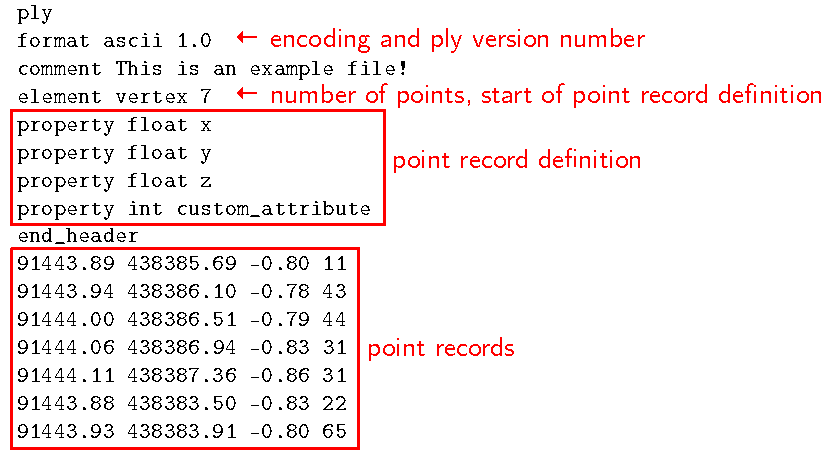
\includegraphics[width=\linewidth]{figs/ply_header.pdf}
  \caption{A simple PLY file with 1 additional user-defined attribute of type integer (\texttt{int}). It contains 7 points.}%
\label{fig:ply}
\end{figure}

%

PLY files are readable by many software packages and can also be stored in a binary encoding\sidenote{\url{https://en.wikipedia.org/wiki/PLY_(file_format)\#ASCII_or_binary_format}}.
Compared to the ASCII encoding, the binary encoding results in a smaller file size and quicker reading and writing from and to the file.
There is no standardised way to specify the CRS in a PLY file, although one could add a comment in the header stating the CRS\@.


%%%
\subsection{The LAS format}%
\index{LAS format}

The \emph{public LASER} (LAS) file format is the most widely used standard for the dissemination of point cloud data.
The LAS standard, currently at version 1.4\marginnote{LAS v1.4 is the latest}, is maintained by the American Society for Photogrammetry and Remote Sensing (ASPRS)  and, as the name implies, it was designed for datasets that originate from (airborne) lidar scanners.
However, in practice it is also used for other types of point cloud, \eg\ those derived from dense image matching.
It is a binary-encoded standard and compared to the PLY format it is rather strict because it prescribes exactly what a point record should look like, \ie\ what attributes are present and how many bits each attribute must use. 

Table~\ref{tab:las-record} shows the composition of the simplest record type that is available for LAS files.
\begin{table*}
  \centering
  \small
  \begin{tabular}{l|l|l|p{7cm}}
    % \toprule
    % \rowcolor[gray]{.9}
    Field & Format & Length (bits) & Description\\ \midrule
    X & int & 32 & X coordinate. \\ 
    Y & int & 32 & Y coordinate. \\ 
    Z & int & 32 & Z coordinate. \\ 
    Intensity & unsigned int & 16 & The pulse return amplitude. \\ 
    Return number & unsigned int & 3 &  The total pulse return number for a given output pulse. \\ 
    Number of returns & unsigned int & 3 & Total number of returns for a given pulse \\ 
    Scan Direction Flag & boolean & 1 & Denotes the direction at which the scanner mirror was travelling at the time of the output pulse. A bit value of 1 is a positive scan direction, and a bit value of 0 is a negative scan direction (where positive scan direction is a scan moving from the left side of the in-track direction to the right side and negative the opposite).  \\ 
    Edge of Flight Line & boolean & 1 & Has a value of 1 only when the point is at the end of a scan. It is the last point on a given scan line before it changes direction. \\ 
    Classification & unsigned int & 5 & Classification code \\ 
    Scan Angle Rank & int & 4 & The angle at which the laser pulse was output from the scanner including the roll of the aircraft. \\ 
    User Data & unsigned int & 4 & May be used at the user's discretion. \\ 
    Point Source ID & unsigned int & 8 & Indicates the file from which this point originated. Non-zero if this point was copied from another file.
    % \bottomrule
  \end{tabular}
\caption{LAS Point Data Record Format 0}%
\label{tab:las-record}
\end{table*}
Other record types are available that also include fields to store for instance  RGB colour information or the GPS time (the time a point was measured by the scanner), but all records types include at least the fields shown in Table~\ref{tab:las-record}.
While the LAS standard clearly specifies that all these fields are required, some of the fields are very specific to lidar acquisition and they are sometimes ignored in practice, \eg\ if a point cloud originating from dense matching is stored in the LAS format.\marginnote{unused fields take up storage} 
It is important to notice that unused fields will still take up storage space in each record.

The CRS of the point cloud can be stored in the header of a LAS file, together with some other general information such as the total number of points and the bounding box of the point cloud. 
The X, Y, and Z fields are stored as 32-bit integers. 
To convert these values to the actual coordinates on the ground, they need to be multiplied by a scaling factor and added to an offset value, \ie:
\begin{gather*}
  X_{coordinate} = (X_{record} * X_{scale}) + X_{offset} \\
  Y_{coordinate} = (Y_{record} * Y_{scale}) + Y_{offset} \\
  Z_{coordinate} = (Z_{record} * Z_{scale}) + Z_{offset}.
\end{gather*}
The scaling factors $X_{scale}$, $Y_{scale}$, $Z_{scale}$ and the offsets $X_{offset}$, $Y_{offset}$, $Z_{offset}$ are also given in the header. Notice that the scaling factor determines the number of decimals that can be stored, \eg\ the factors $0.1$, $0.01$, and $0.001$ would give us $1$, $2$, and $3$ decimals respectively.

The LAS standard defines several classification codes, as listed in Table~\ref{tab:las-classes}.
\begin{table}
  \centering
  \begin{tabular}{l|l}
  % \toprule
  % \rowcolor[gray]{.9}
  Code & Meaning \\ \midrule
  0 & never classified \\
  1 & unclassified \\
  2 & ground \\
  3 & low vegetation \\
  4 & medium vegetation \\
  5 & high vegetation \\
  6 & building \\
  7 & low point (noise) \\
  8 & \emph{reserved} \\
  9 & water \\
  % \bottomrule
\end{tabular}
\caption{The first 10 LAS classification code numbers. More codes exist, but they are not listed here.}%
\label{tab:las-classes}
\end{table}
These codes are to be used as values for the classification field of a point record, and are intended to indicate the type of object a point belongs to.
Which classes are used strongly depends on the dataset at hand.
The codes $0$ and $1$ may appear ambiguous, but there is a clear distinction.
To be exact, the code $0$ is used for points that were never subjected to a classification algorithm, whereas the code $1$ is used for points that have been processed by a classification algorithm, but could not be assigned to a specific class.
It is possible to define your own classes using code ranges that are reserved for that purpose.

%%%
\paragraph{AHN3 classification.} 
The national Dutch AHN3 lidar dataset 
\marginnote{\emph{Actueel Hoogtebestand Nederland} (AHN)}
\marginnote{\url{https://www.ahn.nl}}
is disseminated in the LAZ format (a compressed LAS, see below) and uses the LAS classification codes. 
Figure~\ref{fig:ahn3} shows all the codes that are used in  AHN3. 
\begin{figure*}
  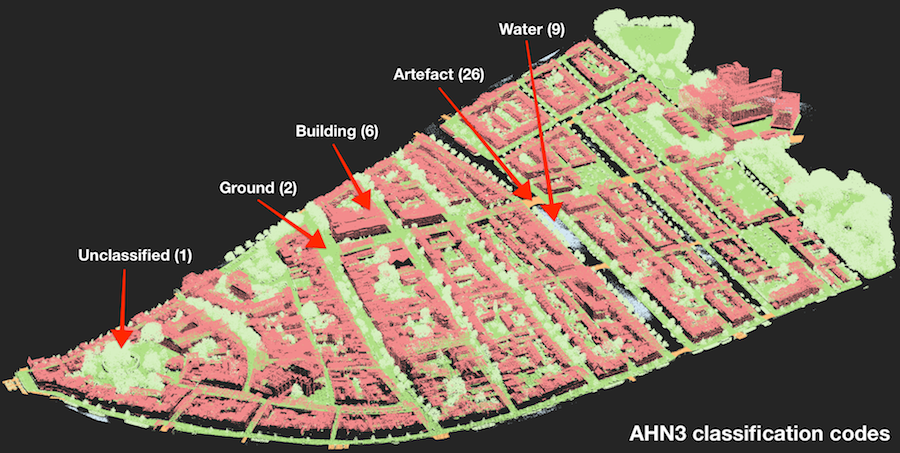
\includegraphics[width=\linewidth]{figs/ahn3.png}
  \caption{Classification codes used in the AHN3 dataset.}%
\label{fig:ahn3}
\end{figure*}
Notice that apart from the pre-defined codes from Table~\ref{tab:las-classes}, it also uses the custom code $26$ for an `artefact' (Dutch: \emph{kunstwerk}) class that includes special infrastructural works such as bridges and viaducts. 

Notice that in AHN3, the points representing vegetation are not classified as such, and vegetation is never explicitly classified.
\marginnote{vegetation is classified as $1$/unclassified in AHN3}
The is because the aim of the AHN project is mostly to model dikes and to protect us from floods, and vegetation is not very important for this use-case.
The class $1$ is thus used for vegetation, but other objects such as street furniture (\eg\ lampposts) or cars are also classified as $1$.


% The standard technically allows for additional user-defined attributes


%%%
\paragraph{The LAZ format.}%
\index{LAZ format}

A compressed variant of the LAS format, dubbed ``LAZ'', exists.
While it is not maintained by an `official' organisation like the LAS standard, it is an open standard and it is widely used, especially for very big dataset.
Through the use of lossless compression algorithms that are specialised for point cloud data, a LAZ file can be compressed into a fraction of the storage space required for the equivalent LAS file, without any loss of information.
This makes it more effective than simply using ZIP compression on a LAS file.
In addition, support for LAZ is typically built into point cloud reading and writing software, so to the user it is no different than opening a LAS file (although the compression and decompression operations do take extra time).

The LAZ format closely resembles the LAS format, \ie\ the header and the structure of the point records are virtually identical.
In a LAZ file the point records are grouped in blocks of 50,000 records each.
Each block is individually compressed, which makes it possible to partially decompress only the needed blocks from a file (instead of always needing to compress the whole file).
This can save a lot of decompression computations if only a few points from a huge point cloud are needed.
Also notice that the effectiveness of the compression algorithms depends on the similarity in information between subsequent point records.
Typically information is quite similar for points that are close to each other in space.
Therefore, a greater compression factor can often be achieved after spatially sorting the points.

In practice, for the AHN3 dataset, the LAZ file of a given area is about 10X more compact than its LAS counterpart.
\marginnote{LAZ = 10X compacter than LAS}
% TODO: add that 10X compacter but also that it's slower to read/write? 
% TODO: and that for AHN3, it's rather essential, since it would be too big otherwise, wouldn't it?

% TODO: speak of zLAS as the devil?


%%%
%
\section{Thinning}%
\label{sec:thinning}
\index{thinning}

A point cloud with fewer points is easier to manage and quicker to visualise and process.
Therefore a point cloud is sometimes \emph{thinned}, which simply means that a portion of the points is discarded and not used for processing.
Commonly encountered thinning methods in practice are:
\begin{itemize}
  \item \textbf{random:} randomly keep a given percentage of the points, \eg\ 10\%.
  \item \textbf{\emph{n}th-point:} keep only the $n$th point in the dataset. For instance, if $n=100$, we would keep the 1st, the 101th, the 201th, etc; a dataset with \qty{100000} points is reduced to \qty{1000} points. This is the quickest thinning method.
  \item \textbf{\emph{n}th-point random:} if there is some structure in the input points (\eg\ if generated from a gridded terrain) then this method could create datasets with artefacts. A variation involves keeping randomly in the $n$ points the point to keep.
  \item \textbf{grid: }overlay a 2D or 3D regular grid over the points and keep $m$ point(s) per grid cell. That can be one of the original points, an average of those, or the exact centre of the cell. The thinning factor depends on the chosen cell-size. Notice that the result is often a point cloud with a homogeneous point density on all surfaces (only on the horizontal surfaces if a 2D grid is used).
\end{itemize}
See Figure~\ref{fig:randvsgrid} for a comparison between random thinning and grid thinning.
\begin{figure}
  \centering
  \begin{subfigure}[b]{0.95\linewidth}
    \centering
    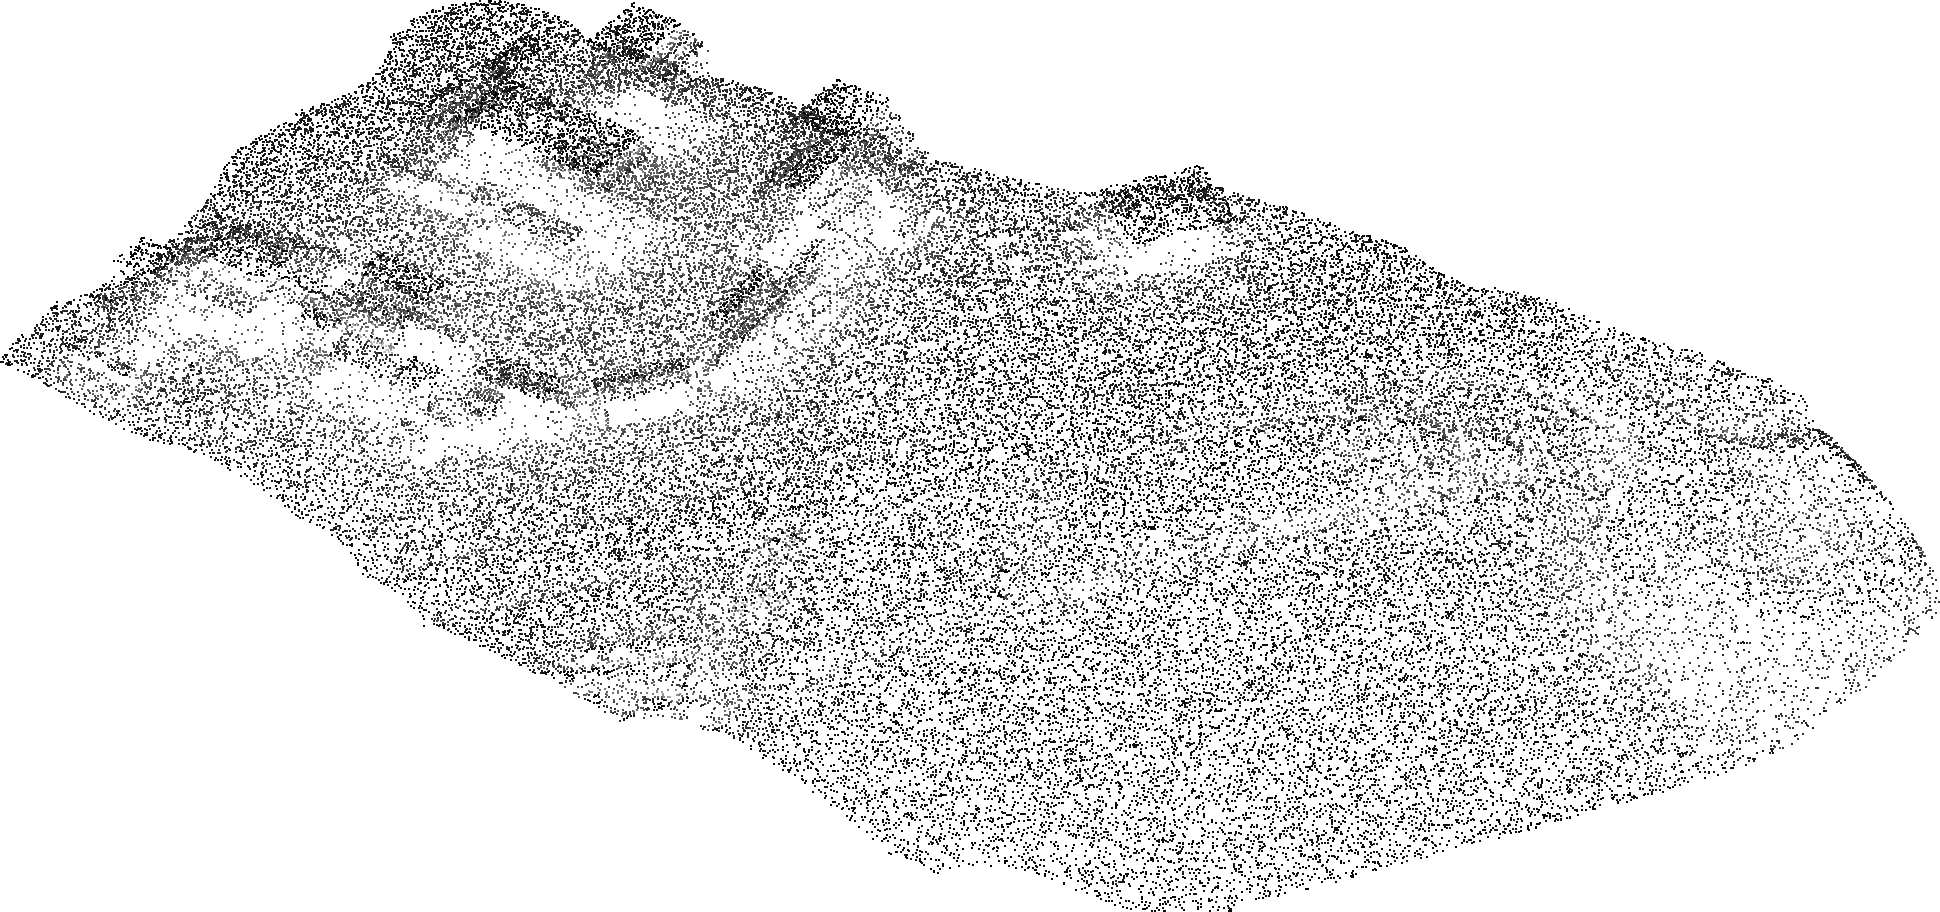
\includegraphics[width=\textwidth]{figs/rand01.png}
    \caption{random thinning}
  \end{subfigure}

  \begin{subfigure}[b]{0.95\linewidth}
    \centering
    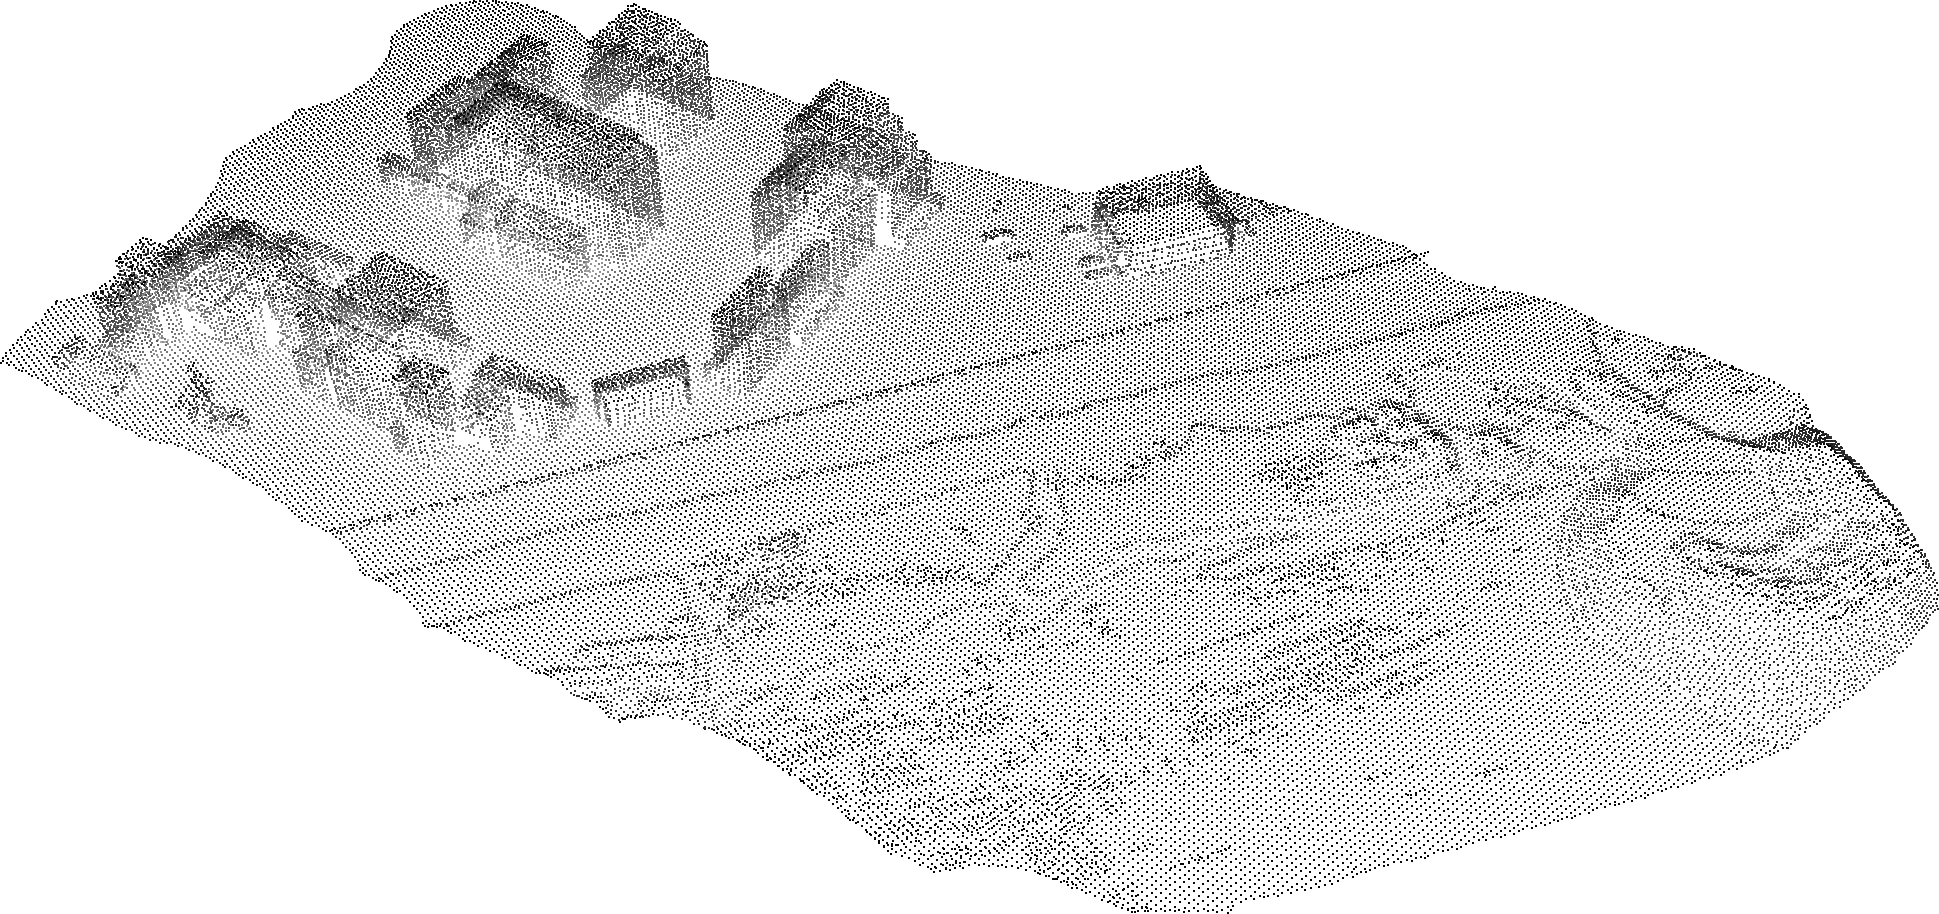
\includegraphics[width=\textwidth]{figs/voxel08m.png}
    \caption{3D grid thinning}
  \end{subfigure}
\caption{Comparison of two thinning methods. The thresholds were chosen such that the number of remaining points is approximately the same.}%
\label{fig:randvsgrid}
\end{figure}

From Section~\ref{sec:tin-simpl} you undoubtedly remember that TIN simplification has a somewhat similar objective: data reduction. 
However, for a given number of resulting points, TIN simplification yields a higher quality end result because it only removes points that are deemed unimportant.
Thinning methods on the other hand do not consider the `importance' of a point in any way, and might discard a lot of potentially meaningful details.
So why bother with thinning? The answer is that thinning methods are a lot faster since they do not require something like a computationally expensive triangulation.
Especially in scenarios where the point density is very high and the available time is limited, thinning can be useful.


%%%
%
\section{Outlier detection}%
\label{sec:outlier_detection}

Recall from Chapter~\ref{chap:acquisition} that outliers are points that have a large error in their coordinates.
Outliers are typically located far away from the terrain surface and often occur in relatively low densities.
Outlier detection aims to detect and remove outliers and is a common processing step for point clouds.

Most outlier detection methods revolve around analysing the local neighbourhood of a point.
The neighbourhood can be defined using a $k$-nearest neighbour (knn) search (see Section~\ref{sec:kdtree}), a fixed radius search, or by superimposing a regular grid on the point cloud and finding the points that are in the same grid-cell.
The points that are determined to be in the neighbourhood of a point of interest $p$ are used to determine whether $p$ is an outlier or not.

The underlying assumption of most outlier detection methods is that an outlier is often an isolated point, \ie\ there are not many points in its neighbourhood. We distinguish the following outlier detection methods (see also Figure~\ref{fig:outlier-detection}):
\begin{figure}[htb]
  \centering
  \begin{subfigure}[b]{0.3\linewidth}
    \centering
    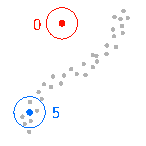
\includegraphics[width=\textwidth]{figs/radius-count.pdf}
    \caption{radius count}
  \end{subfigure}
  \begin{subfigure}[b]{0.3\linewidth}
    \centering
    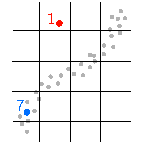
\includegraphics[width=\textwidth]{figs/grid-count.pdf}
    \caption{grid count}
  \end{subfigure}
  \begin{subfigure}[b]{0.3\linewidth}
    \centering
    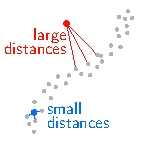
\includegraphics[width=\textwidth]{figs/knn-distance.pdf}
    \caption{knn distance ($k=3$)}
  \end{subfigure}
\caption{Three outlier detection methods based on local point density. The red point is an outlier, whereas the blue point is an inlier.}%
\label{fig:outlier-detection}
\end{figure}

\begin{itemize}
  \item \textbf{radius count:} Count the number of points that are within a fixed radius from $p$. If the count is lower than a given threshold, $p$ is marked as an outlier.
  \item \textbf{grid count:} Superimpose a grid on the point cloud and count for each grid-cell the number of points. If the count is lower than a given threshold, the points inside the corresponding grid cell are marked as outliers. Sometimes the neighbourhood is extended with adjacent grid cells. The grid method has the advantage that it can be used with the spatial streaming paradigm (see Section~\ref{sec:streaming}).
  \item \textbf{knn distance:} Find the $k$ nearest neighbours of $p$, \eg\ using a $k$d-tree, and compute the mean or median of the distances between $p$ and its neighbours. If this value is above a given threshold, $p$ is marked as an outlier.
\end{itemize}

These methods generally work well if the outliers are isolated.
However, in some cases this assumption does not hold.
For example in case of a point cloud derived from multi-beam echo sounding (see Section~\ref{sec:acquisistion-techniques}), a common issue is the occurrence of (shoals of) fish. 
These fish cause large groups of points that are clustered closely together above the seafloor.
These are not isolated points since each outlier will have plenty of other points nearby.
A possible solution is to construct a TIN of all points and to `cut' the relatively long edges that connect the outlier clusters to the seafloor.
This splits the TIN into several smaller TINs, and the largest of those should then be the seafloor surface without the outliers. 
Figure~\ref{fig:mbes} gives an example.
\begin{figure*}
  \centering
  \begin{subfigure}[b]{0.44\linewidth}
    \centering
    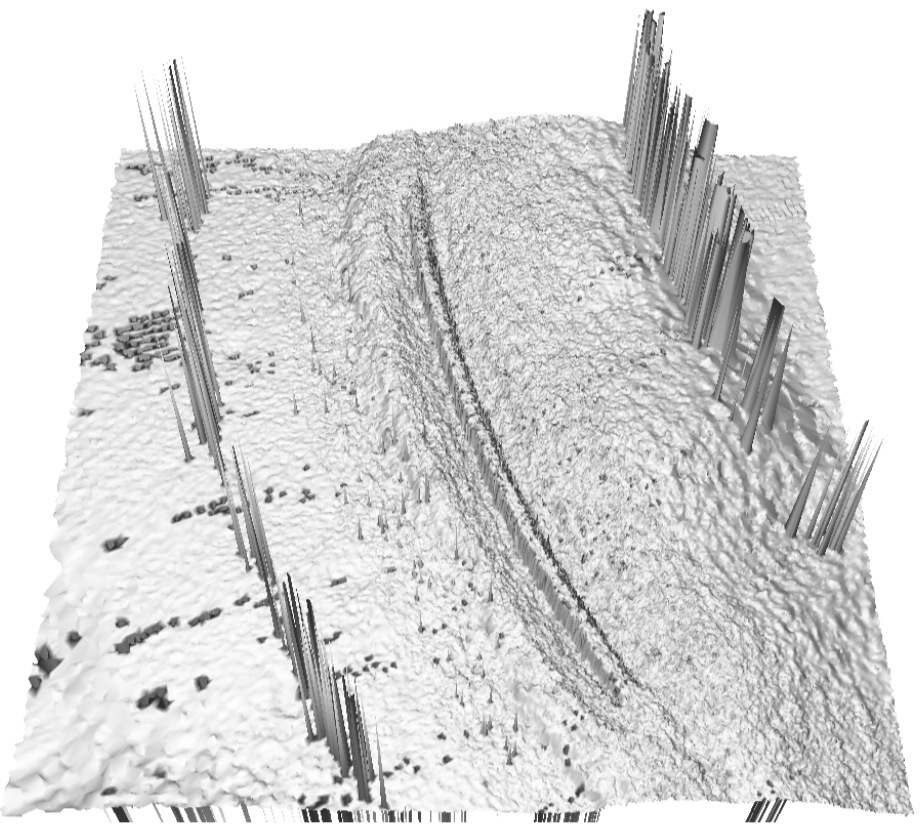
\includegraphics[width=\textwidth]{figs/mbes_cleaning_before.png}
    \caption{before outlier detection}
  \end{subfigure}
  \qquad%
  \begin{subfigure}[b]{0.44\linewidth}
    \centering
    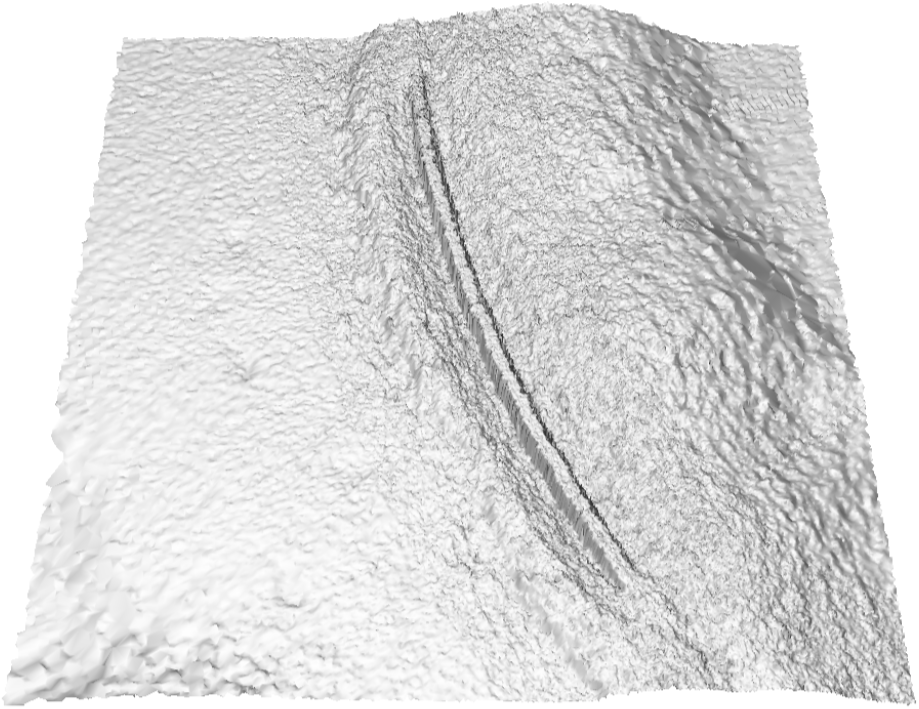
\includegraphics[width=\textwidth]{figs/mbes_cleaning_after.png}
    \caption{after outlier detection}
  \end{subfigure}
\caption{Outlier detection in a multi-beam echo sounding dataset using a TIN \citep{Arge10}.}%
\label{fig:mbes}
\end{figure*}
% TODO: shouldn't we use our own figure here?


%%%%%%%%%%%%%%%%%%%%
%

\section{Ground filtering}
Ground filtering involves classifying the points of a point cloud into ground points and non-ground points.
Ground points are those points that are part of the bare-earth surface of the earth, thus excluding vegetation and man-made structures such as buildings and cars.
The ground points can then be used to generate a DTM, usually as a TIN or a raster.
Or, the non-ground points can be used as input for another classifier, \eg\ to classify buildings and vegetation possibly using a region growing algorithm (see Section~\ref{sec:regiongrowing}).

Ground filtering methods are typically based on the assumptions that 
\begin{enumerate}
  \item the ground is a continuous surface without sudden elevation jumps, 
  \item for a given 2D neighbourhood, the ground points are the ones with the lowest elevation.
\end{enumerate}
Notice that outliers (especially those under the ground surface) may break these assumptions and in some cases it may be necessary to first run an outlier removal algorithm such as that in Section~\ref{sec:outlier_detection}. (see \eg\ Figure~\ref{fig:axelsson:profiles}).


% TODO: shouldn't we use our own figure here?
\begin{figure}
  \centering
  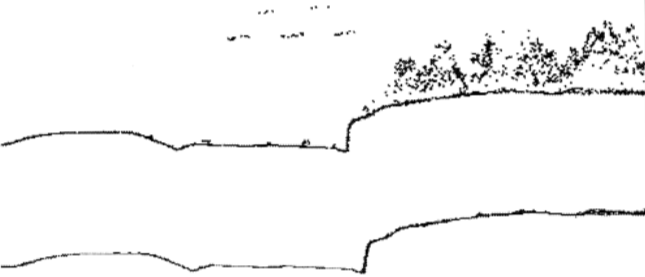
\includegraphics[width=0.8\textwidth]{figs/axelsson-profiles.png}
  \caption{Cross-section of a terrain with lamp posts and trees before (top) and after (bottom) ground filtering \citep{axelsson2000generation}.}%
\label{fig:axelsson:profiles}
\end{figure}

Notice that the resulting bare-earth model may thus have holes where these non-ground objects used to be.
If needed, these holes can be filled in a subsequent processing step involving spatial interpolation.

%%%
%
\subsection{Ground filtering with TIN refinement}%
\index{ground filtering}

We will now discuss an effective ground filtering method that is based on the \emph{greedy} insertion of ground points into a TIN\@.
Indeed, the same algorithmic paradigm of iterative TIN refinement that we saw earlier in Section~\ref{sec:tin-simpl} is used.
The algorithm consists of three main steps:
\begin{enumerate}
  \item construction of a rudimentary initial TIN (usually a Delaunay TIN);
  \item computation of two geometric properties for each point that is not already labelled as ground;
  \item incremental insertion of points that pass a simple and local `ground test' based on the computed geometric properties.
\end{enumerate}
The latter two steps are repeated until all remaining points fail the ground test.

In the first step a rudimentary initial TIN is constructed from a number of points that have locally the lowest elevation and are spread somewhat evenly over the data extent.
These points are found by superimposing a 2D grid over the data extent and by selecting the lowest point for each grid cell (similar to grid thinning).
The cell-size of the grid should be chosen such that it is larger than the largest non-ground object (usually a building).
Thus, if the largest building has a footprint of 100mX100m, the cellsize should be a bit larger, \eg\ \qty{110}{m}, so that it is guaranteed that each grid-cell has at least a few ground points.
Each point that is inserted into the TIN is considered to be a ground point.

In the second step two geometric properties are computed for each point that was not added to the TIN\@.
These properties are based on the relation between the point $p$ and the triangle in the current TIN that intersects its vertical projection. 
The two properties are illustrated in Figure~\ref{fig:ground-filtering:symbols}.
\begin{figure*}
  \centering
  \begin{subfigure}[b]{0.25\linewidth}
    \centering
    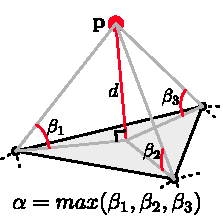
\includegraphics[width=\textwidth]{figs/groundfilter-symbols.pdf}
    \caption{}\label{fig:ground-filtering:symbols}
  \end{subfigure}
  \begin{subfigure}[b]{0.25\linewidth}
    \centering
    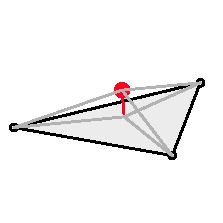
\includegraphics[width=\textwidth]{figs/groundfilter-ground.pdf}
    \caption{example ground point}\label{fig:ground-filtering:ground}
  \end{subfigure}
  \begin{subfigure}[b]{0.25\linewidth}
    \centering
    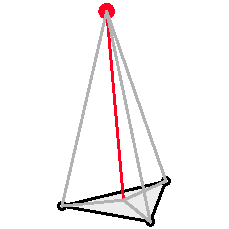
\includegraphics[width=\textwidth]{figs/groundfilter-nonground.pdf}
    \caption{example non-ground point}\label{fig:ground-filtering:nonground}
  \end{subfigure}
  \caption{Geometric properties for a point $p$ in the method for ground filtering based on TIN refinement.}%
\label{fig:ground-filtering}
\end{figure*}
The first property, denoted $d$, is the perpendicular distance between the $p$ and the plane spanned by the triangle.
The second property, denoted $\alpha$, is the largest angle of the angles between the triangle and the three vectors that connect each vertex with $p$. 

In the ground test of the final step, it is simply checked for each point if its $d$ is below a given threshold $d_{\max}$ and if its $\alpha$ is below a given threshold $\alpha_{\max}$.
If this is indeed the case, the point is labelled as a ground point and inserted into the TIN\@.
Compare Figures~\ref{fig:ground-filtering:ground} and~\ref{fig:ground-filtering:nonground}.

Of course, if the triangles in the TIN change, the properties of the overlapping unclassified points need to be recomputed. 
However, the algorithm is greedy, which means that it never ``goes back'' on operations that were previously performed, and thus  when a point $p$ is inserted as the ground, it is never removed.
When all remaining points fail the ground test, the algorithm terminates.
Figure~\ref{fig:axelsson} gives an example result.
\begin{figure*}
  \centering
  \begin{subfigure}[b]{0.48\linewidth}
    \centering
    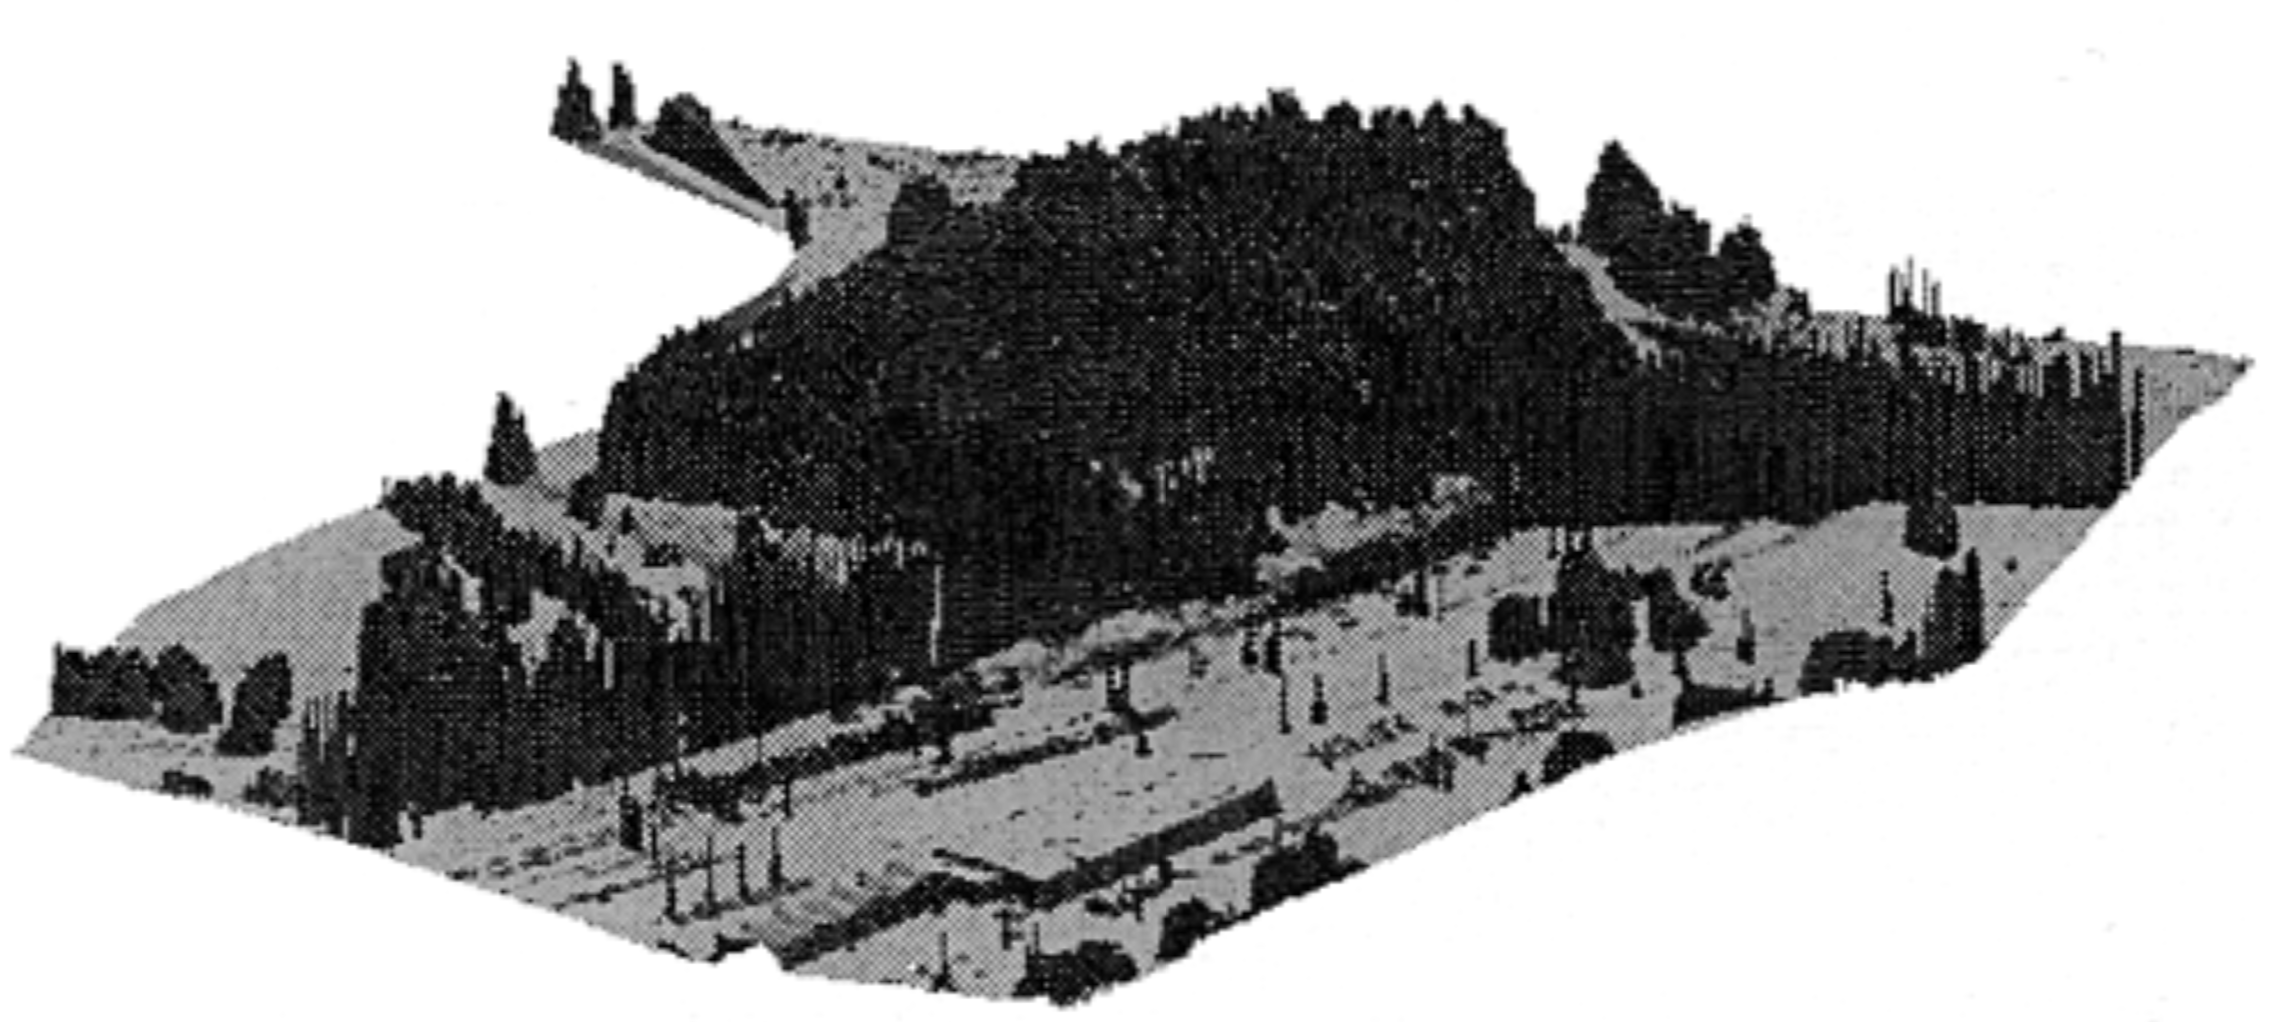
\includegraphics[width=\textwidth]{figs/axelsson-before.png}
    \caption{Before}
  \end{subfigure}
  \quad
  \begin{subfigure}[b]{0.48\linewidth}
    \centering
    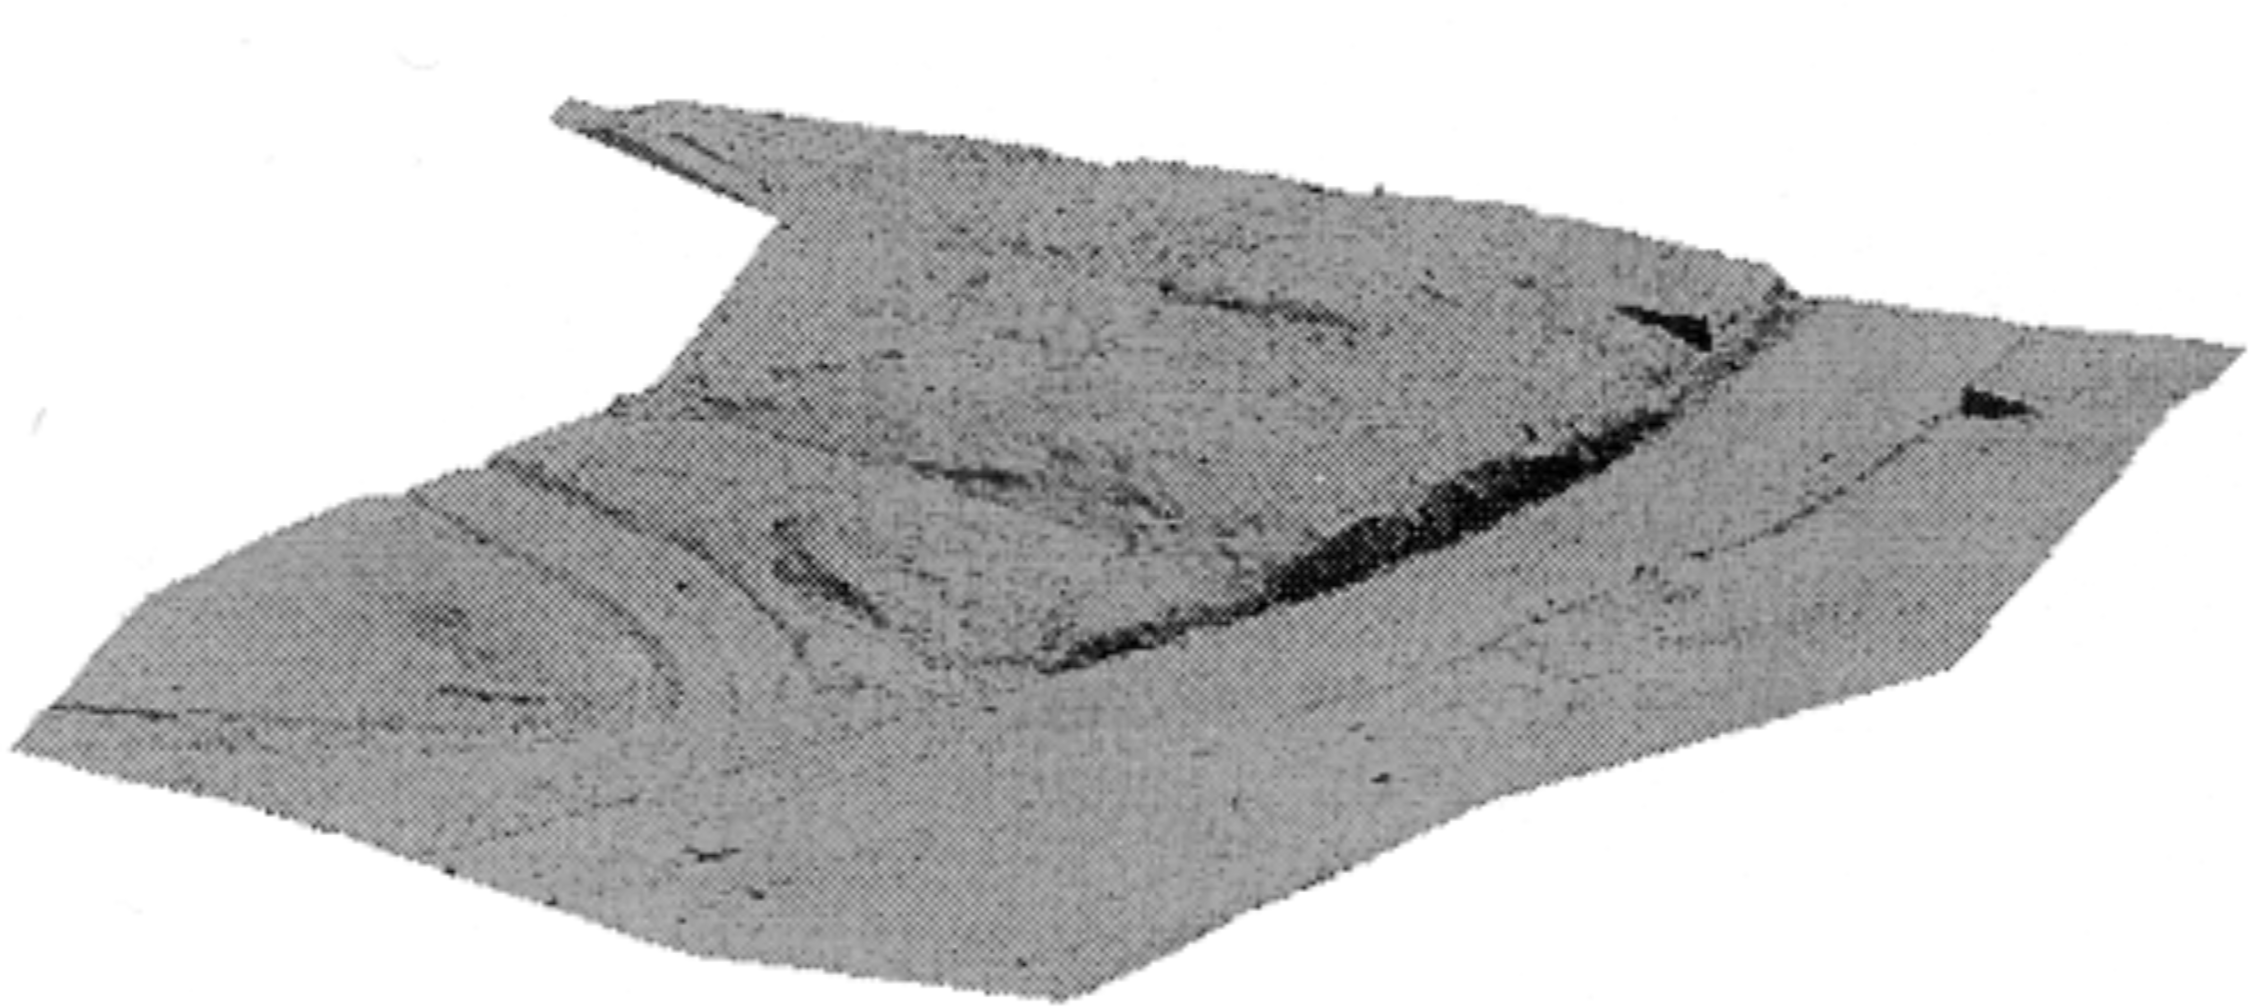
\includegraphics[width=\textwidth]{figs/axelsson-after.png}
    \caption{After}
  \end{subfigure}
\caption{Ground filtering \citep{axelsson2000generation}}%
\label{fig:axelsson}
\end{figure*}

\paragraph{Time complexity.} The worst case time complexity is $\mathcal{O}(n^2)$, since the most expensive term is related to the last two steps of the algorithm; for each of the $n$ points we need to do the ground test, and after each test we need to recompute the geometric properties of at most $n$ points.


%%%
%
\subsection{Cloth simulation filter (CSF) algorithm}

An alternative to TIN refinement is the algorithm called \emph{Cloth simulation filter} (CSF).
Unlike the previous one, no TIN is required, its input is only a point cloud.
The main observation necessary for this algorithm is that lower points are usually forming the ground (again it is assumed no outliers appear below the ground in the dataset).

%

The key idea of the algorithm, as shown in Figure~\ref{fig:csf_idea},
\begin{figure*}
  \centering
  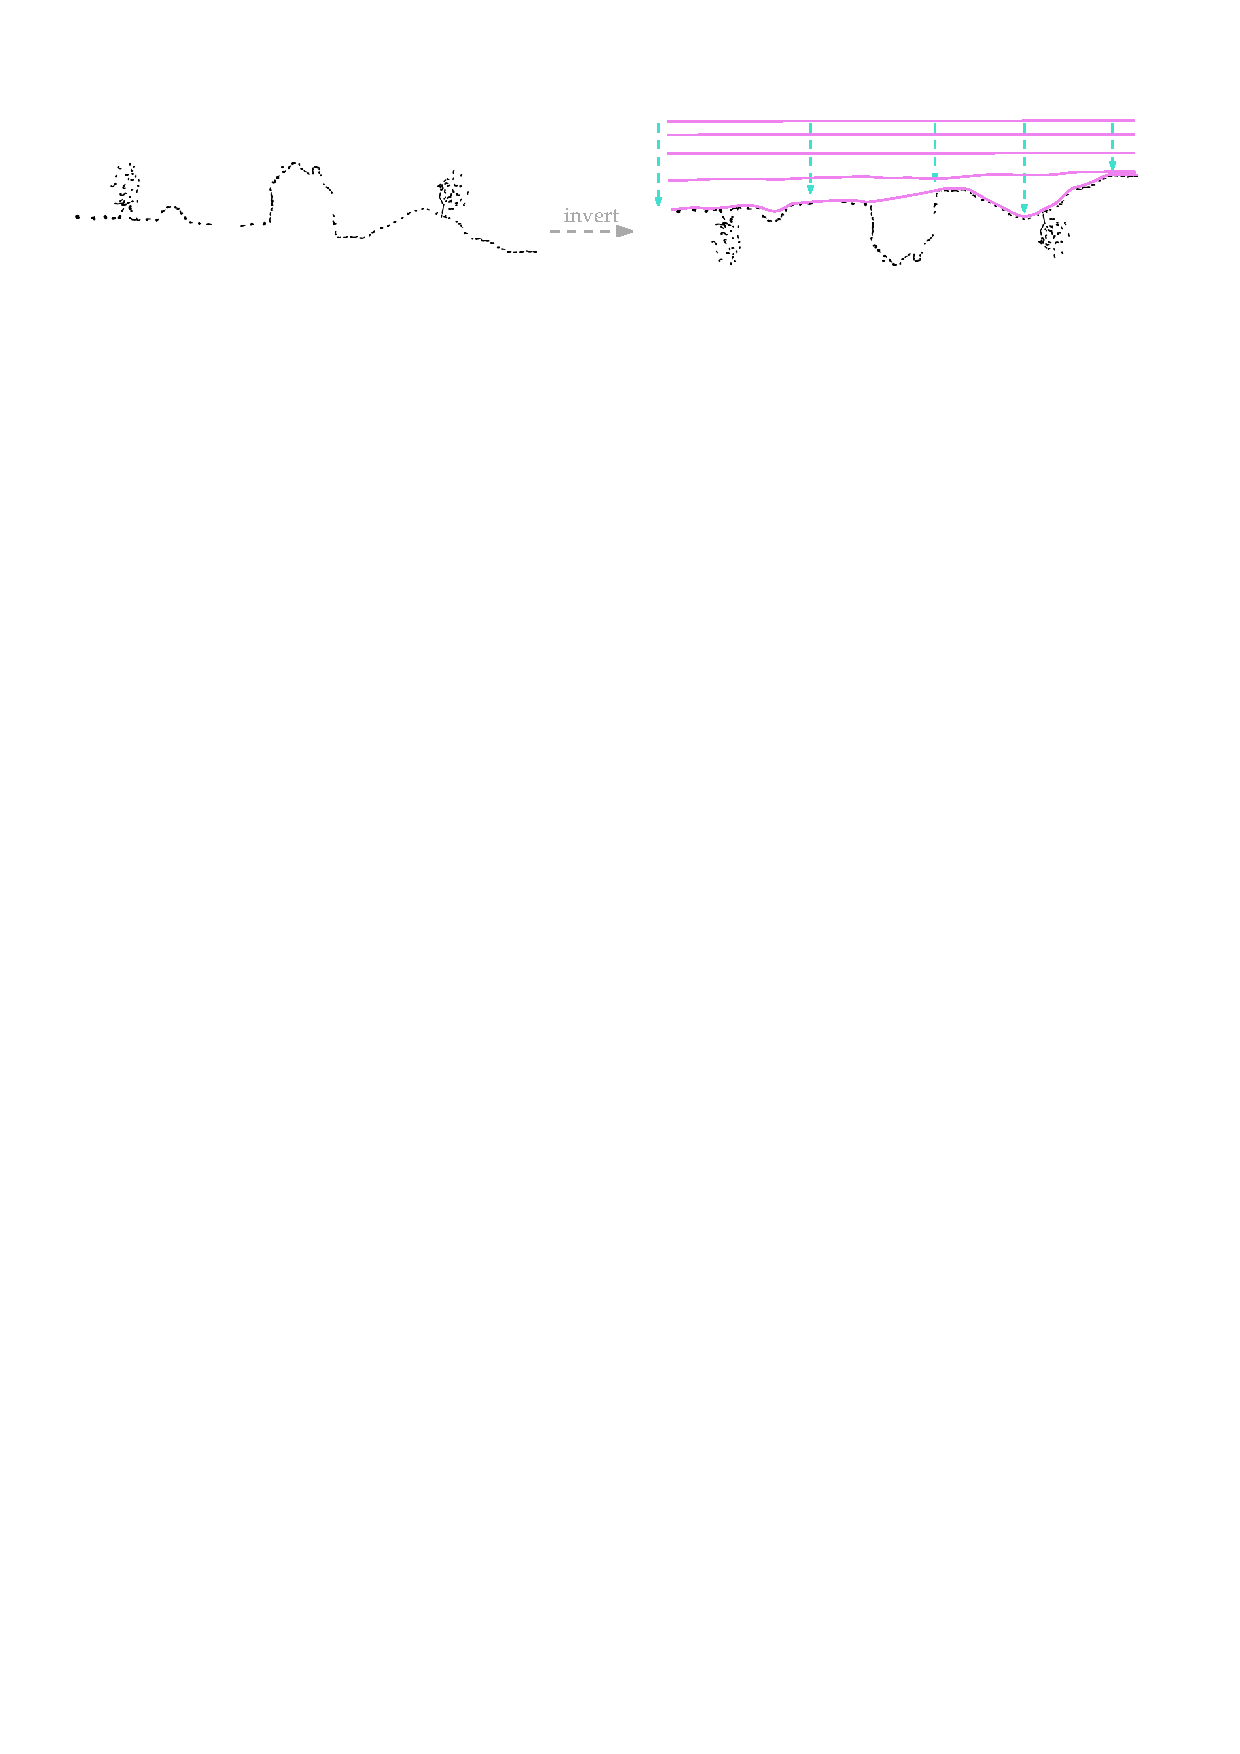
\includegraphics[width=0.95\linewidth]{figs/csf_idea}
  \caption{Basic idea behind the CSF algorithm for ground filtering of a point cloud: inverting the data and letting a cloth fall.}%
\label{fig:csf_idea}
\end{figure*}
is to invert (upside-down) a point cloud, and to let a piece of cloth fall from the sky.
The cloth will fall until it reaches the points forming the ground.
During the process, we aim to control the \emph{tension} (or rigidity) of the cloth, so that areas where there is no sample point, or where there are large buildings, can be filled realistically.

%

The CSF algorithm is a simplification of an algorithm in computer graphics to simulate a piece of cloth falling on an object.
The cloth is modelled as a surface formed of \emph{particles} (vertices) that are regularly distributed on a grid, these particles have a mass and they are connected to their neighbours (4-neighbours in this case).
For terrains (2.5D objects), the particles are constrained to only move vertically.

Two factors influence the $z$-value of a particle during the cloth falling process:
\begin{enumerate}
  \item \textbf{external forces:} in this case this is the gravity pulling down a particle;
  \item \textbf{internal forces:} the tension in the cloth, which is modelled by the interactions between a particle and its neighbours.
\end{enumerate}
As particles fall down, some will reach the ground and become \emph{unmovable}.
These will potentially be neighbours to \emph{movable} ones, whose elevation will be controlled by how we define the rigidity of the cloth.

As shown in Figure~\ref{fig:csf_iterations},
\begin{marginfigure}
  \centering
  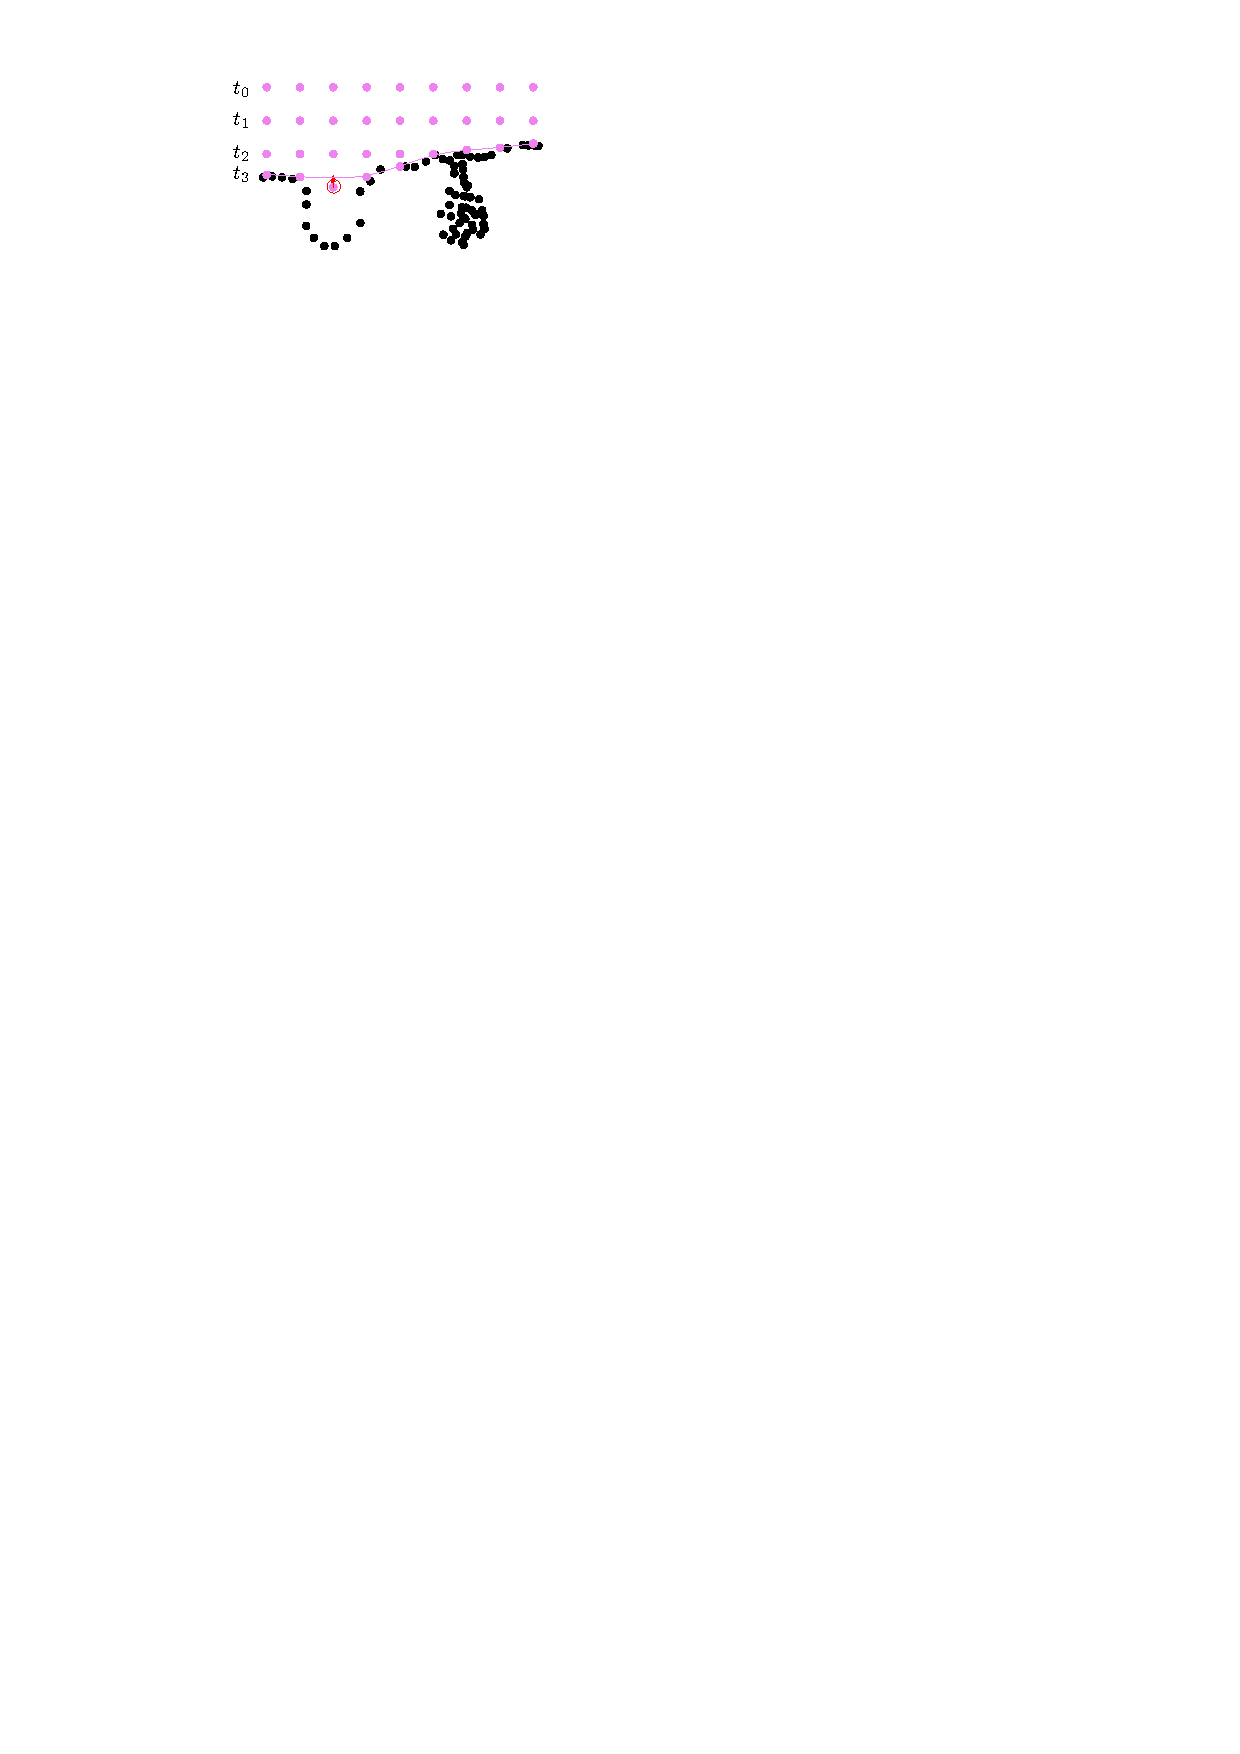
\includegraphics[width=\linewidth]{figs/csf_iterations}
  \caption{}%
\label{fig:csf_iterations}
\end{marginfigure}
the process is iterative. We first define a cloth formed of particles, and then for each iteration we calculate the next $z$-value of each particle based on the vector of displacement from the external and internal forces at the previous step.
If a particle is movable (\ie\ it has not reached the ground yet), then the gravity force is applied (a vector pointing downwards; its magnitude will depend on the momentum of the particle) and afterwards the internal forces are applied.
Notice that in Figure~\ref{fig:csf_iterations}, the particle in red at $t_3$ was moved downwards because of the gravity, but its internal forces are a vector pointing upwards since its 2 neighbours (it would be 4 for a 2D case) are have higher $z$-values.

The algorithm is detailed in Algorithm~\ref{algo:csf}.
\begin{algorithm} 
  \DontPrintSemicolon\
  \KwIn{A set $S$ of sample points from a point cloud;\\ 
  resolution $r$ of the cloth grid;\\ 
  tolerance $\epsilon_{zmax}$ to stop the iterations\\
  tolerance $\epsilon_{ground}$ to classify points in $S$}
  \KwOut{The points in $S$ are classified as ground/non-ground}
  invert $S$ \;
  initialise the cloth $C$ at an elevation $z_0$ higher than the highest elevation \;
  \For{all $p \in C$} 
  {
    $p_{zmin} =$ lowest possible elevation based on $S$ \nllabel{l:zmin} \;
    $p_{zprev} = z_0 + displacement$ \nllabel{l:init_prev}\;
    $p_{zcur} = z_0$ \;
  }
  % \tcc{initialise the cloth $C$}
  \While{$\Delta z > \epsilon_{zmax}$}
  {
    \tcc{external forces}
    \For{all $p \in C$} 
    {
      \If{$p$ is movable}
      {
        tmp = $p_{zcur}$ \;
        $p_{zcur} = (p_{zcur} - p_{zprev}) + p_{zcur}$ \;
        $p_{zprev} = tmp$ \;
      }
    }
    \tcc{internal forces, process once each pair $e$ of adjacent particles}
    \For{all $e \in C$}
    {
      $p0 = e_{start}$ \;
      $p1 = e_{end}$ \;
      update $p0_{zcur}$ and $p1_{zcur}$ if they are movable \;
    } 
    \tcc{calculate the max $\Delta z$}
    \For{all $p \in C$}
    {
      \If{$(p_{zcur} - p_{zprev}) > \Delta z$}
      {
        $\Delta z = (p_{zcur} - p_{zprev})$ \;
      }
    }
  }
  \caption{CSF algorithm}%
\label{algo:csf}
\end{algorithm}

%

\paragraph{Initialisation of the cloth.}
The cloth is first initialised at an arbitrary height above the highest points are the point cloud.
The cloth is formed of particles regularly distributed according to a user-defined parameter.
We assume that all particles have the same mass, and we define arbitrarily a first displacement vector due to the gravity (pointing downwards) (line~\ref{l:init_prev}).
For each particle $p$, we need to define the lowest elevation it can move, once it reaches it it is labelled as unmovable (line~\ref{l:zmin}).
The lowest elevation of one particle $p$ is defined as the original elevation of the closest sample point $s$ after projecting both to the 2D-plane.

%

\paragraph{How the process ends.}
This iterative process is repeated until the maximum displacement of all particles is less than a user-defined parameters ($\epsilon_{zmax}$); or until a certain number of iterations has been performed.

%

\paragraph{Internal forces.}
The internal forces are applied only to movable particles; once a particle has been labelled as unmovable it cannot be moved again.
Given a movable particle $p$, we apply the internal forces by individually looking at its 4 neighbours $n_i$.
For each neighbour $n_i$, there are two cases (see Figure~\ref{fig:csf_2cases}):
\begin{marginfigure}
  \centering
  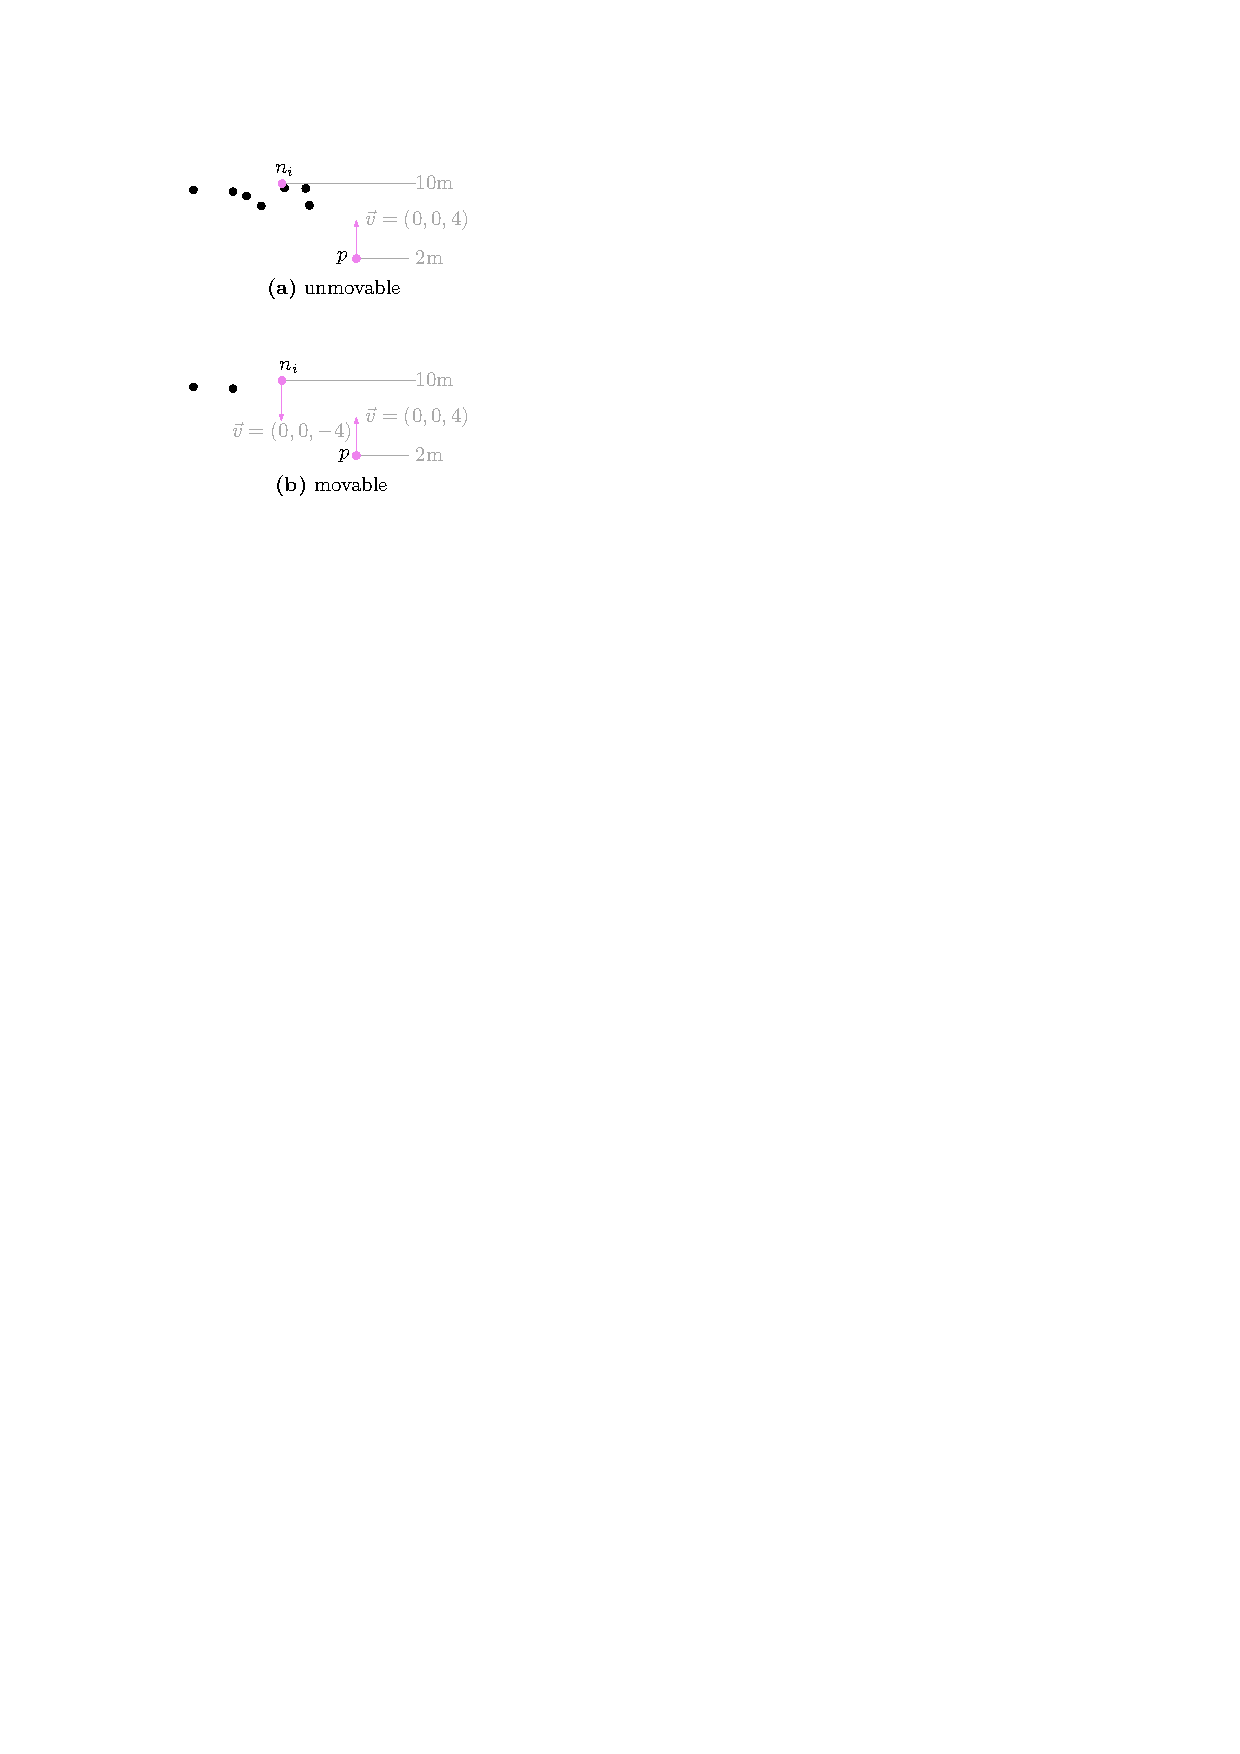
\includegraphics[width=\linewidth]{figs/csf_2cases}
  \caption{}%
\label{fig:csf_2cases}
\end{marginfigure}
\begin{enumerate}
  \item \textbf{$n_i$ is unmovable:} only $p$ is moved, towards $n_i$. 
  \item \textbf{$n_i$ is movable:} the idea is that both $p$ and $n_i$ will try to move towards each other to the same height. The vector applied to each will thus be in opposite direction. 
\end{enumerate}

\paragraph{Controlling the tension/rigidity.}
Notice that in Figure~\ref{fig:csf_2cases}b, both particles are moved to the same elevation, but that it is also possible to scale the internal forces displacement vector, \eg\ to 0.8 of its length (and thus decrease the tension in the cloth). Lower internal force displacement means that the particles will move more during a single iteration and so the tension in the cloth is effectively reduced. 
The same idea applies to Figure~\ref{fig:csf_2cases}a, the displacement vector can be controlled by scaling the displacement vector. 
In Figure~\ref{fig:csf_2cases} it is 0.5 of the difference in elevation, but if less tension is wanted, then the scale could be for instance 0.4 (so that the movable particle has an internal displacement $\vec{v}=(0, 0, 3.2)$, because $0.4 * (10-2) = 3.2$) or 0.3.

% TODO: order dependent

\paragraph{Output: a ground surface +  classification of points.}

When the process is completed, the surface of the cloth can be used as an approximation of the bare-earth (it is possible to triangle it or to create a grid from it).
If a segmentation/classification of the input points is wanted, then the distance between a sample point of the original point cloud and the cloth can be used: if this distance is less than a given user-defined threshold then the sample point is a ground point.

\begin{floatbox}
  \begin{kaobox-practice}[frametitle=\faCog\ CSF is implemented in several open-source libraries]
  The description of the CSF algorithm in this book is a simplification of the original algorithm (see \citet{Zhang16}), it omits the post-processing to take into account steep slopes.
  \\ \\
  The complete algorithm is available in the open-source software \emph{CloudCompare} (\url{https://cloudcompare.org}) and in the open-source library \emph{PDAL} (\url{https://pdal.io}).
  \end{kaobox-practice}
\end{floatbox}


%%%
%
\section{Shape detection}%
\label{sec:shape-detection}%
\index{shape detection}

\begin{figure*}
	\centering
	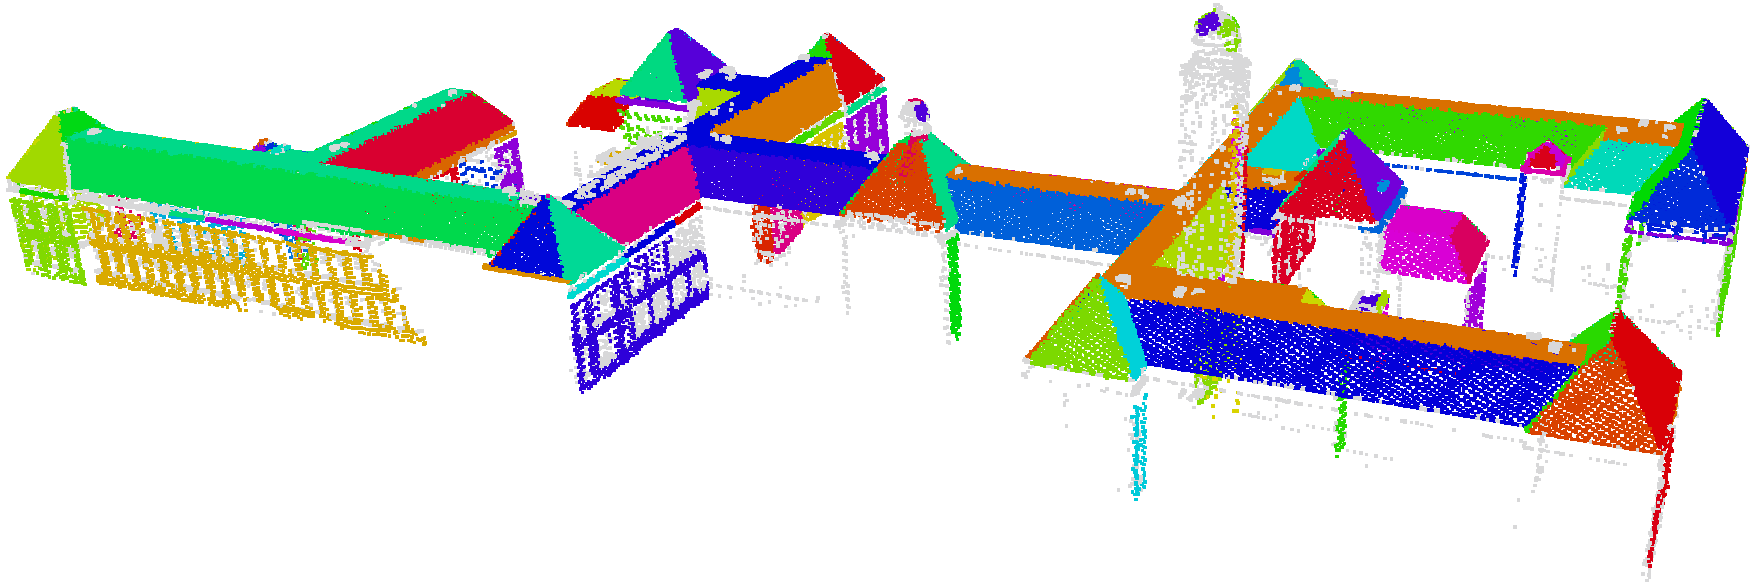
\includegraphics[width=\linewidth]{figs/bk-planes.png}
	\caption{Planar regions in the AHN3 point cloud. Each region was assigned a random colour.}%
\label{fig:bk-planes}
\end{figure*}

Using shape detection we are able to automatically detect simple shapes such as planes in a point cloud.
See for example Figure~\ref{fig:bk-planes}, where the points are randomly coloured according to the corresponding planar surfaces.
Shape detection is an important step in the extraction and reconstruction of more complex objects, \eg\ man-made structures such as buildings are often composed of planar surfaces.

In this section, three shape detection methods will be introduced: 
\begin{enumerate}
  \item RANSAC, 
  \item region growing, 
  \item Hough transform.
\end{enumerate}


But, first we will declare some common terminology.
Let $P$ denote a point cloud. 
If we perform shape detection on $P$ we aim to find a subset of points $S \subset P$ that fit with a particular shape. 
Most shape detection methods focus on shapes that can be easily parametrised, such as a line, a plane, or a sphere. 
If we specify values for the parameters of such a parametrised shape, we define an \emph{instance} of that shape.
A line for example can be parametrised using the equation $y = mx + b$, in this case $m$ and $b$ are the parameters.
We can create an instance of a line by specifying values for its parameters $m$ and $b$, respectively fixing the slope and the position of the line.

In the following, the methods are described in a general way, \ie\ without specialisations for one particular shape.
Only for illustrative purposes specific shapes such as a line or a plane are used to (visually) explain the basic concept of each shape detection method, but the same could be done with spheres, cones, or other shapes.


%In the following we will focus on plane detection  and discuss three different methods that can do that.

%The shapes are represented using a
%A prerequisite for a shape to be suitable for most shape detection methods, is that it has a simple mathematical model.
%A line for example can mathematically be represented with a point and a vector, so can a plane, and circles and spheres can be represented with a point and radius.
%When point is said to support 
%Segmentation is the process of grouping point clouds into multiple homogeneous regions with similar properties.
%% Precisely what similarity properties to use depends on your goal.
%A popular application of segmentation is the detection of planar regions in a point cloud.
%In this case the point cloud is segmented into groups of points that each correspond to a plane.
%This can be helpful for something like building classification, if we assume that buildings consist of planar surfaces.

%%%
\subsection{RANSAC}%
\index{RANSAC}
% how does it work, pseudocode

RANSAC is short for \emph{RANdom SAmpling Consensus} and as its name implies it works by randomly sampling the input points.
In fact it starts by picking a random set of points $M \subset P$. 
This set $M$ is called the \emph{minimal set}\index{minimal set}\marginnote{minimal set} and contains exactly the minimum number of points that is needed to uniquely construct the shape that we are looking for, \eg\ 2 for a line and 3 for a plane. 
From the minimal set $M$ the (unique) shape instance $\mathcal{I}$ is constructed (see Figures~\ref{fig:ransac:b} and~\ref{fig:ransac:c}).
\begin{figure}
	\centering
	\begin{subfigure}[b]{0.24\linewidth}
		\centering
		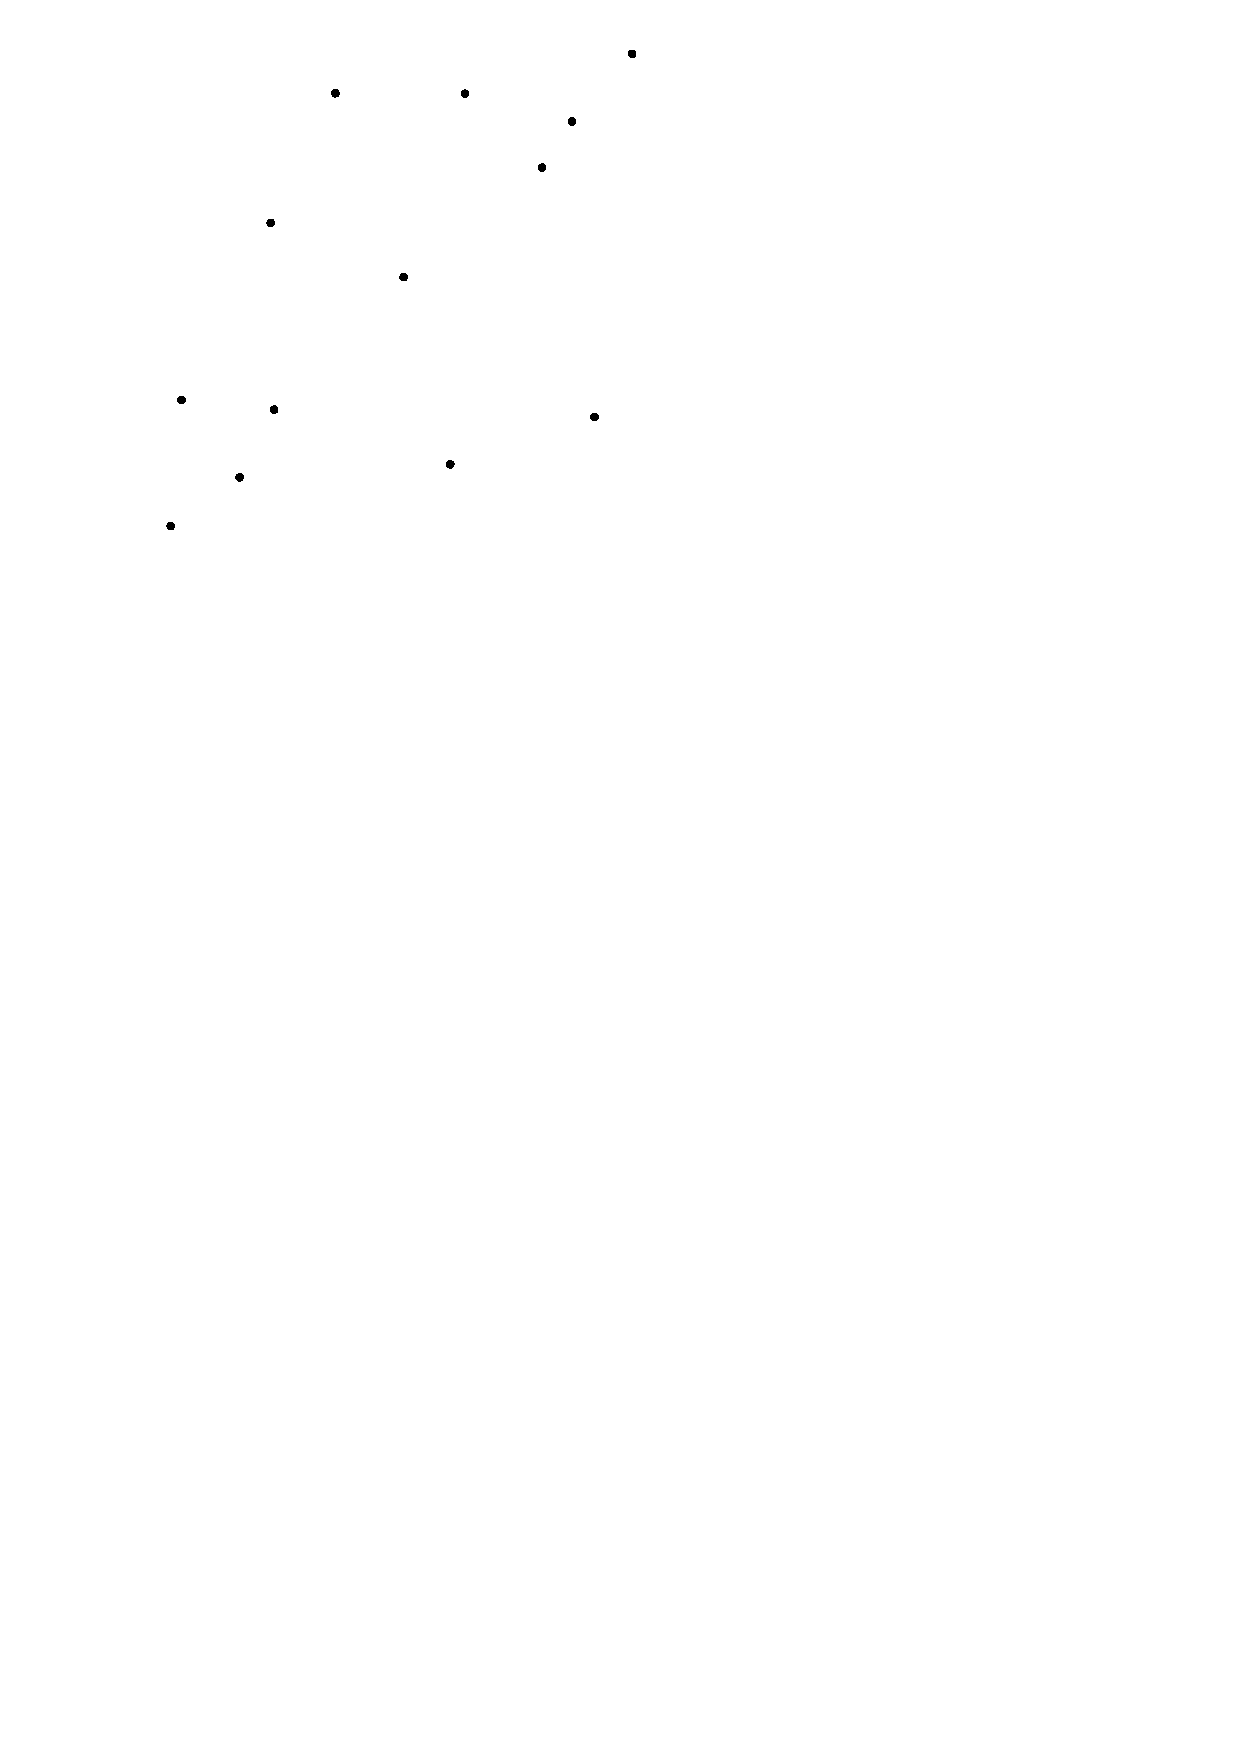
\includegraphics[width=\textwidth,page=1]{figs/ransac.pdf}
		\caption{Input points}\label{fig:ransac:a}
	\end{subfigure}
	\begin{subfigure}[b]{0.24\linewidth}
		\centering
		\includegraphics[width=\textwidth,page=2]{figs/ransac.pdf}
		\caption{First minimal set}\label{fig:ransac:b}
	\end{subfigure}
	\begin{subfigure}[b]{0.24\linewidth}
		\centering
		\includegraphics[width=\textwidth,page=3]{figs/ransac.pdf}
		\caption{Second minimal set}\label{fig:ransac:c}
	\end{subfigure}
	\begin{subfigure}[b]{0.24\linewidth}
		\centering
		\includegraphics[width=\textwidth,page=4]{figs/ransac.pdf}
		\caption{Detected line instance}\label{fig:ransac:d}
	\end{subfigure}
	\caption{RANSAC for line detection ($k=2$ iterations)}%
\label{fig:ransac}
\end{figure}
The algorithm then checks for each point $p \in \{P \setminus M\}$ if it fits with $\mathcal{I}$. 
This is usually done by computing the distance $d$ from $p$ to $\mathcal{I}$ and comparing $d$ against a user-defined threshold $\epsilon$.
If $d<\epsilon$ we say that $p$ is an \emph{inlier}\index{inlier}\marginnote{inlier}, otherwise $p$ is an outlier.
The complete set of inliers is called the \emph{consensus set}\index{consensus set}\marginnote{consensus set}, and its size is referred to as the \emph{score}\index{score}\marginnote{score}.
The whole process from picking a minimal set to computing the consensus set and its score, as shown in Algorithm~\ref{algo:ransac}, is repeated a fixed number of times, after which the shape instance with the highest score is outputted (Figure~\ref{fig:ransac:d}). 

\begin{algorithm}
	\KwIn{An input point cloud $P$, the error threshold $\epsilon$, the minimal number of points needed to uniquely construct the shape of interest $n$, and the number of iterations $k$}
	\KwOut{the detected shape instance $\mathcal{I}_{best}$}
	$s_{best} \leftarrow 0$\;
	$\mathcal{I}_{best} \leftarrow$ nil\;

	\For{$i \leftarrow 0 \ldots k$}
	{
		$M \leftarrow n$ randomly selected points from $P$\;
		$\mathcal{I} \leftarrow$ shape instance constructed from $M$\;
		$C \leftarrow \emptyset$ \;
		\For{all $p \in P \setminus M$} 
		{
			$d \leftarrow$ distance$(p,\mathcal{I})$\;
			\If{$d < \epsilon$}{
				add $p$ to $C$\;
			}
		}
		$s \leftarrow$ score$(C)$\;
		\If{$s > s_{best}$}{
			$s_{best} \leftarrow s$ \;
			$\mathcal{I}_{best} \leftarrow \mathcal{I}$\;
		}
	}
	\caption{The RANSAC algorithm}%
\label{algo:ransac}
\end{algorithm}


%Refit? Minimum size consensus set. Different evaluation than score

% parameter tuning and probablity of finding a good solution...

% pros and cons
The most touted benefit of RANSAC is its robustness, \ie\ its performance in the presence of many outliers (up to 50\%). 
Other algorithms to identify planes, \eg\ fitting a plane with least-square adjustment, are usually more sensitive to the presence of noise and outliers (which are always present in real-world datasets).
The probability that a shape instance is detected with RANSAC depends mainly on two criteria:
\begin{enumerate}
	\item the number of inliers in $P$, and
	\item the number of iterations $k$.
\end{enumerate}
Naturally, it will be easier to detect a shape instance in a dataset with a relatively low number of outliers.
And it is more likely that a shape instance is found if more minimal sets are evaluated.
Picking a sufficiently high $k$ is therefore important for the success of the algorithm, although a higher $k$ also increases the computation time.
%With the right parameters it can detect shapes in point clouds with up to 50\% outliers.

Because of the random nature of RANSAC, the minimal sets that it will evaluate will be different every time you run the algorithm, even if the input data is the same.
The detected shape instance can therefore also be different every time you run the algorithm; RANSAC is therefore said to be a \emph{non-deterministic} algorithm.
This could be a disadvantage.

\paragraph{Time complexity.} The time complexity of RANSAC is $\mathcal{O}(kn)$, where $n$ is the size of $P$.

%Another disadvantage is that RANSAC can output spurious results in some cases. This is shown in Figure~\ref{fig:ransac-spurious} where RANSAC found a plane 
%\begin{figure}
%	\centering
%	\includegraphics[width=0.8\textwidth]{figs/ransac-spurious.png}
%	\caption{Detection of a spurious plane by RANSAC \citep{Limberger15}.}
%	\label{fig:ransac-spurious}
%\end{figure}
%- can detect shapes in wrong places, eg. single lidar scanline is perfectly planar.  Eg if there is a set of seemingly arbitrarily coplanar points that is larger than the  set of points corresponding to the smallest plane you want  to detect, than it is more likely to detect the false plane.


\subsection{Region growing}%
\label{sec:regiongrowing}%
\index{region growing}

Region growing works by gradually growing sets of points called \emph{regions} that fit a particular shape instance.
A region $R$ starts from a \emph{seed point}\index{seed point}\marginnote{seed point}, \ie\ a point that is suspected to fit a shape instance.
More points are added to $R$ by inspecting \emph{candidate points}, \ie\ points in the neighbourhood of the members of $R$.
To check if a candidate point $c$ should be added to $R$, a test is performed.
In the case of region growing for plane detection (see Figure~\ref{fig:region-growing}) this test entails computing the angle between the normal vector of $c$ and the normal vector\sidenote{The normal vector for a point $p\in P$ can be found by fitting a plane to the points in the local neighbourhood of $p$. The vector orthogonal to this plane is the normal vector.} of its neighbour in $R$.
If this angle is small it is assumed that $c$ lies in the plane instance that corresponds to $R$, and that it can therefore be added to $R$.
Otherwise $c$ is ignored (Figure~\ref{fig:region-growing:d}).
\begin{figure*}
	\centering
	\begin{subfigure}[b]{0.3\linewidth}
		\centering
		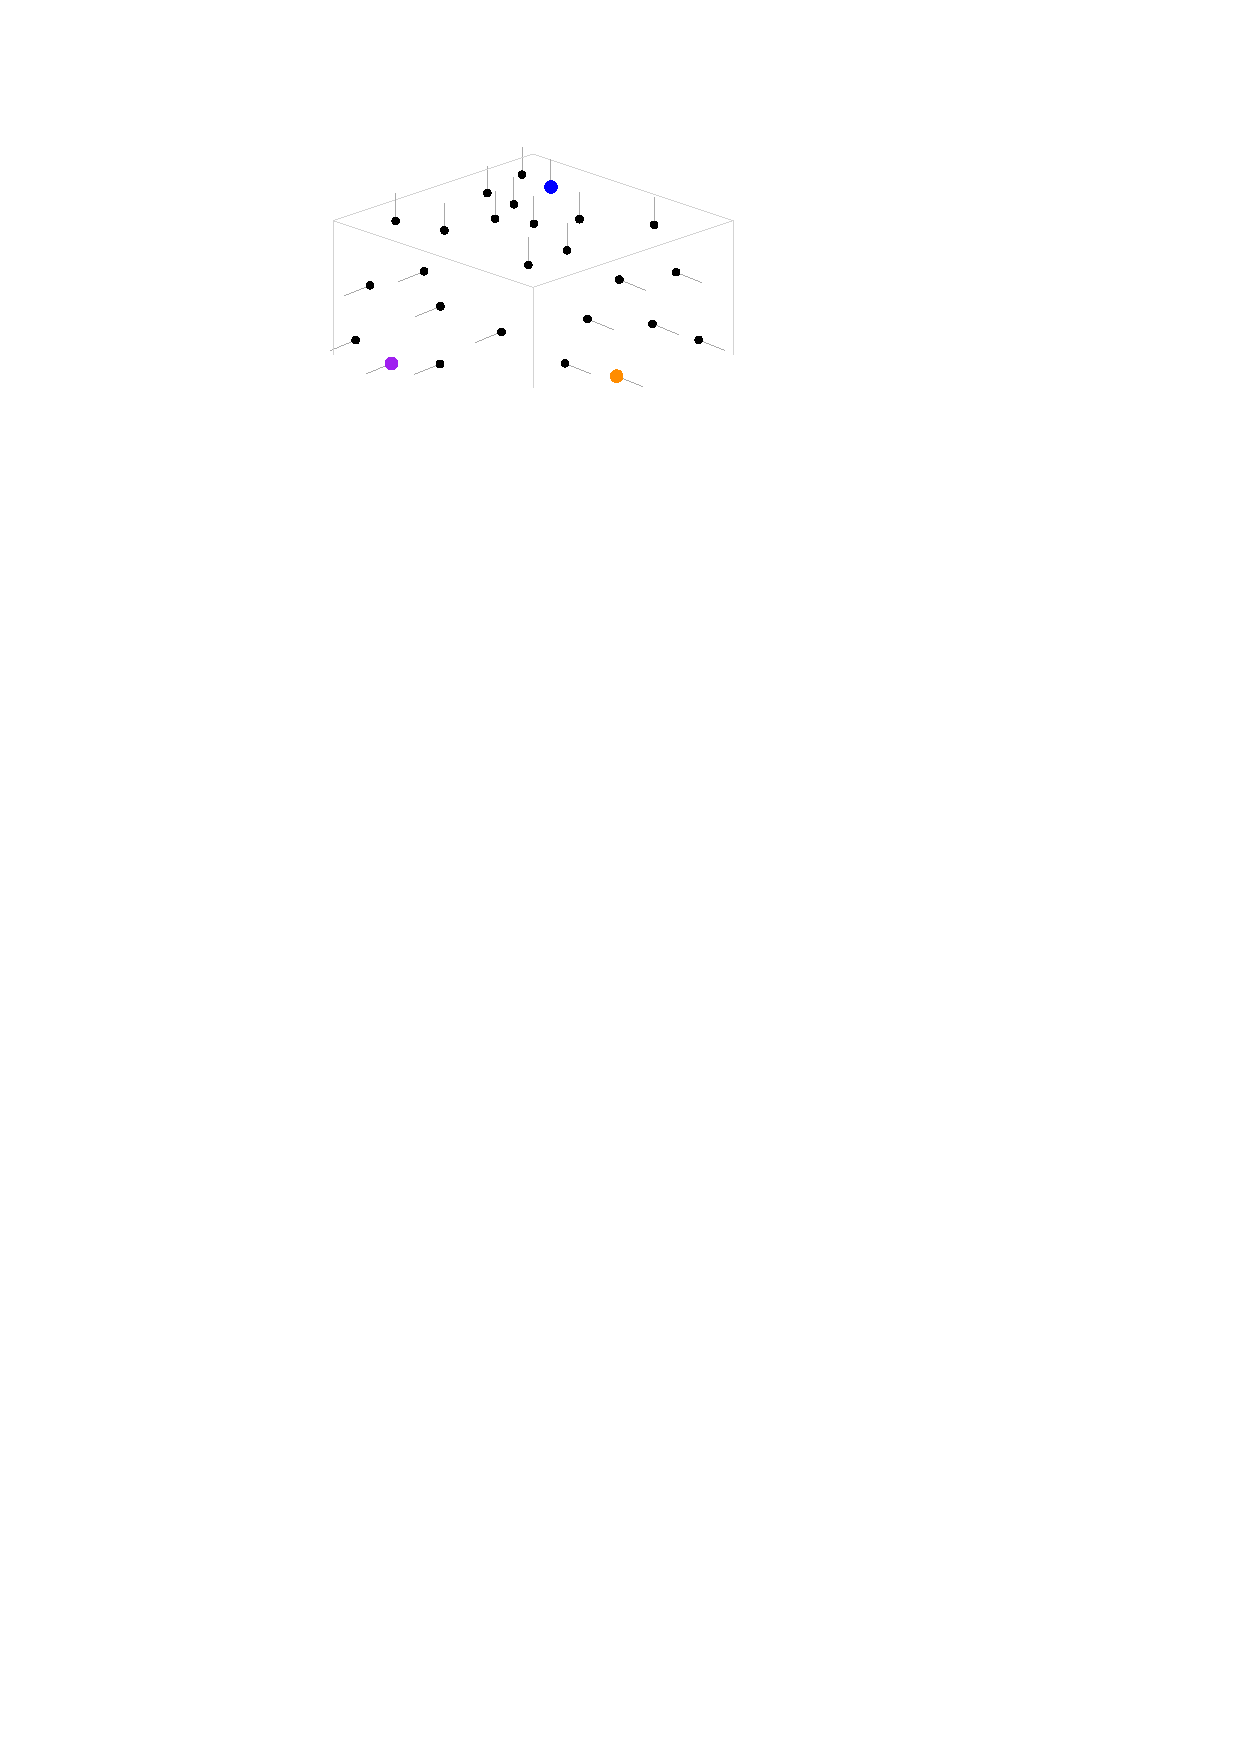
\includegraphics[width=\textwidth,page=1]{figs/region-growing.pdf}
		\caption{Input points with normals and three seed points}\label{fig:region-growing:a}
	\end{subfigure}
	\qquad
	\begin{subfigure}[b]{0.3\linewidth}
		\centering
		\includegraphics[width=\textwidth,page=2]{figs/region-growing.pdf}
		\caption{Start growing. Add neighbours if the normal angle is small.}\label{fig:region-growing:b}
	\end{subfigure}
	\qquad
	\begin{subfigure}[b]{0.3\linewidth}
		\centering
		\includegraphics[width=\textwidth,page=3]{figs/region-growing.pdf}
		\caption{Continue growing from new region point}\label{fig:region-growing:c}
	\end{subfigure}
	\begin{subfigure}[b]{0.3\linewidth}
		\centering
		\includegraphics[width=\textwidth,page=4]{figs/region-growing.pdf}
		\caption{Stop growing where the normal angle is too great}\label{fig:region-growing:d}
	\end{subfigure}
	\qquad
	\begin{subfigure}[b]{0.3\linewidth}
		\centering
		\includegraphics[width=\textwidth,page=5]{figs/region-growing.pdf}
		\caption{Final regions from all three seed points}\label{fig:region-growing:e}
	\end{subfigure}
	\caption{Region growing for plane detection based on the angle between neighbouring point normals}%
\label{fig:region-growing}
\end{figure*}
This process of growing $R$ continues until no more candidates can be found that are compatible with $R$.
When this happens, the algorithm proceeds to the next seed point to grow a new region.

Algorithm~\ref{algo:region-growing} gives the pseudo-code for the region growing algorithm.
Notice that the set $S$ is used to keep track of the points in the current region whose neighbours still need to be checked.
Also notice that candidate points that are already assigned to a region are skipped.
\begin{algorithm}
	\KwIn{An input point cloud $P$, a list of seed points $L_S$, a function to find the neighbours of a point $neighbours()$}
	\KwOut{A list with detected regions $L_R$}
	
	$L_R \leftarrow [\xspace]$\;
	\For{each $s$ in $L_S$} {
		$S \leftarrow \{s\}$\;
		$R \leftarrow \emptyset$\;
		\While{$S$ is not empty}
		{
			$p \leftarrow $ pop$(S)$\;
			\For{each candidate point $c \in$ neighbours$(p)$} 
			{
				\If{$c$ was not previously assigned to any region} {
					\If{$c$ fits with $R$}{
						add $c$ to $S$\;
						add $c$ to $R$\;
					}
				}
			}
		}
		append $R$ to $L_R$\;
	}
	\caption{The Region growing algorithm}%
\label{algo:region-growing}
\end{algorithm}

The seed points can be generated by assessing the local neighbourhood of each input point. 
For example in case of plane detection one could fit a plane through each point neighbourhood and subsequently sort all points on the fitting error. 
Naturally, points with a low plane fitting error are probably part of a planar region so we can expect them to be good seeds.

To compute the point neighbourhoods a k-nearest neighbour search or a fixed radius search can be used, which can both be implemented efficiently using a $k$d-tree (see Section~\ref{sec:kdtree}).
Notice that region growing is based on the idea that we can always find a path of neighbouring points between any pair of points within the same region.
This does mean that two groups of points that fit the same shape instance but are not connected through point neighbourhoods will end up in different regions.
Other shape detection methods described in this chapter do not need point neighbourhood information.

% pros and cons
%- normal estimation is unreliable around corners and affected by noise
%- segmentation that goes around a corner to include  points that still lier within the e-band
%-/+ depends on point neighbourhood
%+ flexible, it can work without a very explicit shape model, eg curved surfaces
\paragraph{Time complexity.} If we assume that 
\begin{enumerate}
	\item the number of seeds in $L_{S}$ is linear with $n$, \ie\ the size of $P$,
	\item the size of $S$ is at most $n$, and that
	\item a $k$nn search takes $\mathcal{O}{(k\log{n})}$, where $k$ is the number of neighbours,
\end{enumerate}
we come to a worst-case time complexity of $\mathcal{O}(n^2k\log{n})$.
In practice it should be better since $S$ is not likely to be $n$ large, and it will get smaller the more regions have been found.


\subsection{Hough transform}%
\index{Hough transform}

The Hough transform uses a voting mechanism to detect shapes.
It lets every point $p \in P$ vote on each shape instance that could possible contain $p$.
Possible shape instances thus accumulate votes from the input points.
The detected shape instances are the ones that receive the highest number of votes.
To find the possible shape instances for $p$, the algorithm simply checks all possible parameter combinations that give a shape instance that fits with $p$.

It is thus important to choose a good parametrisation of the shape that is to be detected.
For instance when detecting lines one could use the slope-intercept form, \ie\ $y = mx+b$. 
However, this particular parametrisation can not easily represent vertical lines, because $m$ would need become infinite which is computationally difficult to manage. 
A better line parametrisation is the Hesse normal form\index{Hesse normal form}\marginnote{Hesse normal form} which is defined as 
\[
r = x\cos{\phi} + y\sin{\phi}. 
\]
As illustrated in Figure~\ref{fig:hough-transform:a} $(r,\phi)$ are the polar coordinates of the point on the line that is closest to the origin, \ie\ $r$ is the distance from the origin to the closest point on the line, and $\phi \in [0^\circ, 180^\circ]$ is the angle between the positive $x$-axis and the line from the origin to that closest point on the line. 
This parametrisation has no problems with vertical lines (\ie\ $\phi=90^{\circ}$).
Similarly, for plane detection we can use the parametrisation
\[
r = x \cos{\theta} \sin{\phi} + y \sin{\phi} \sin{\theta} + z \cos{\phi}.
\]
Where $(r, \theta, \phi)$ are the spherical coordinates of the point on the plane that is closest to the origin.

Figure~\ref{fig:hough-transform} shows an example for line detection with the Hough transform and Algorithm~\ref{algo:hough-transform} gives the full pseudo-code.
\begin{figure*}
	\centering
	\begin{subfigure}[b]{0.3\linewidth}
		\centering
		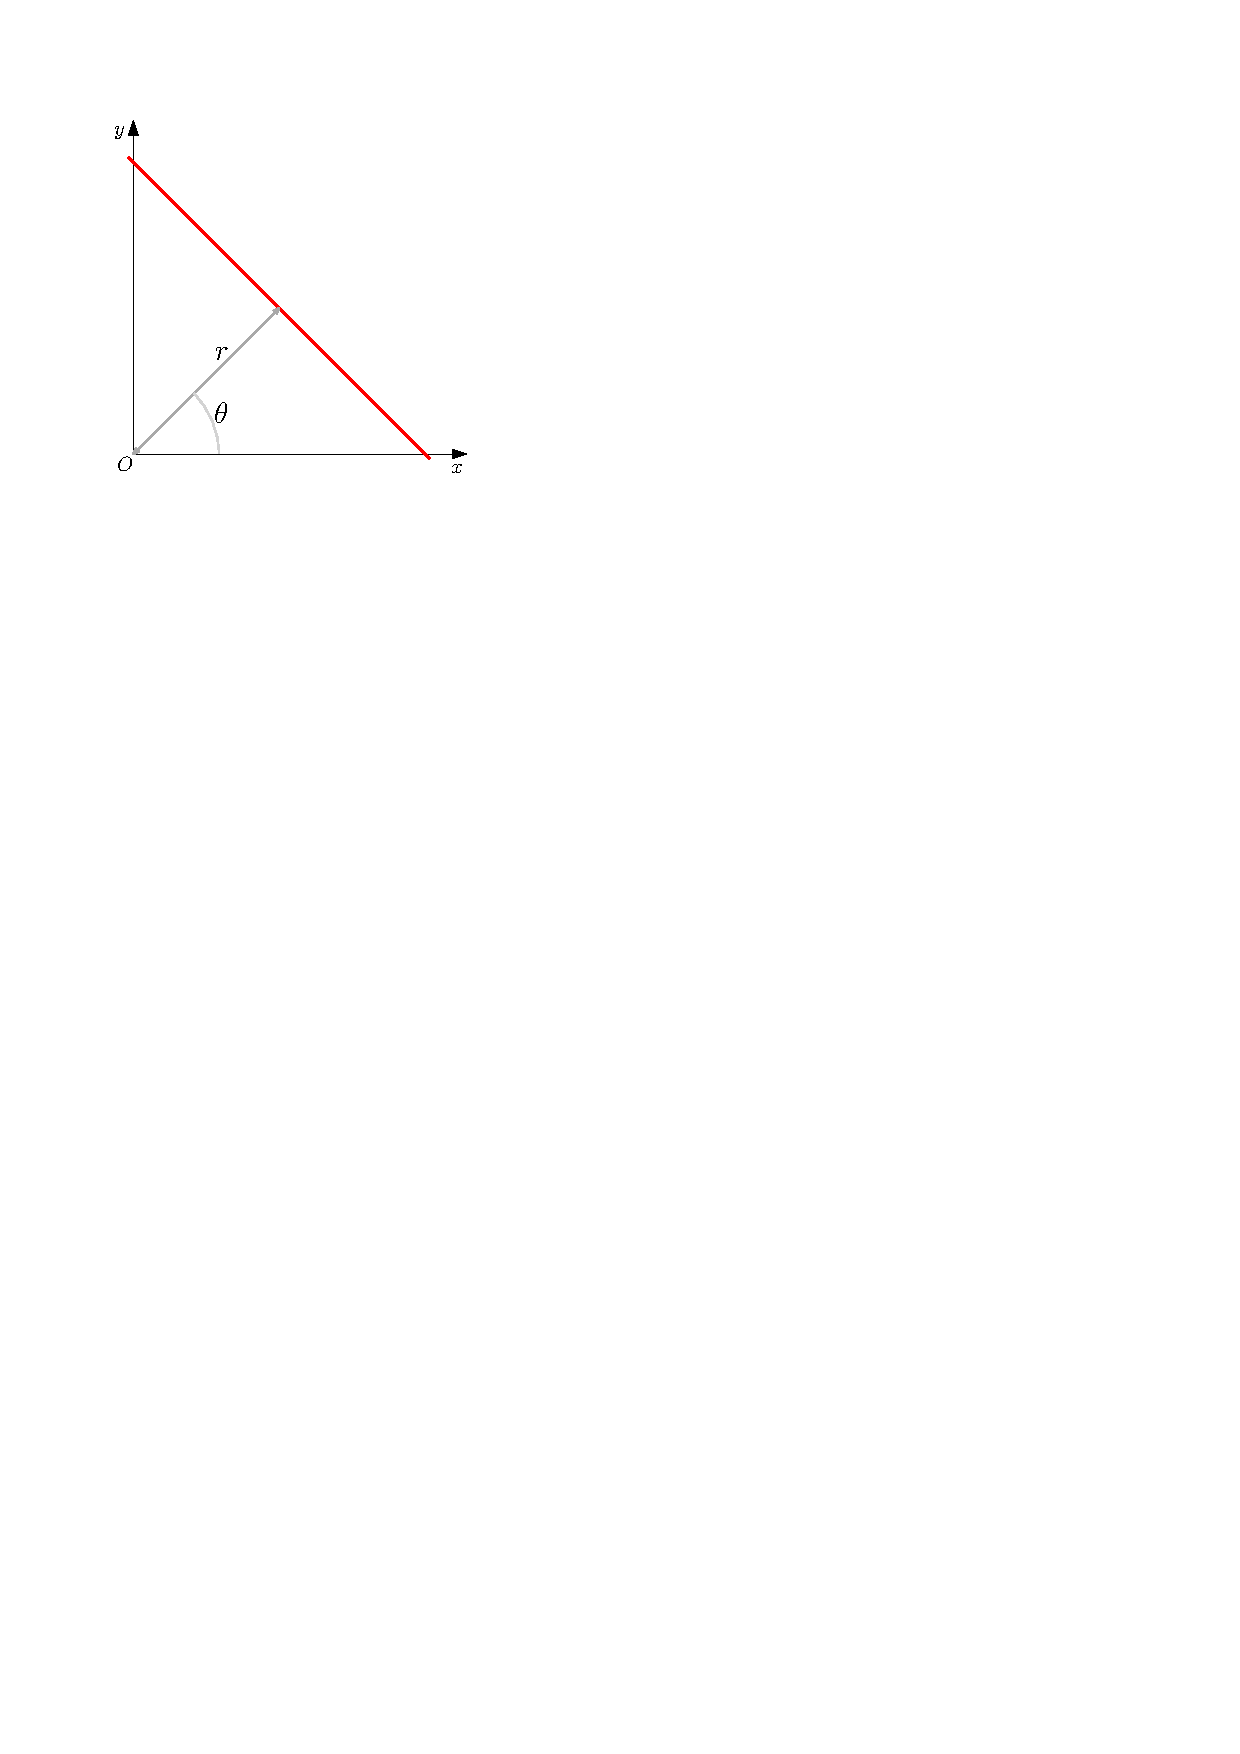
\includegraphics[width=\textwidth,page=1]{figs/hough-transform.pdf}
		\caption{Line parametrisation}\label{fig:hough-transform:a}
	\end{subfigure}
	\qquad
	\begin{subfigure}[b]{0.3\linewidth}
		\centering
		\includegraphics[width=\textwidth,page=2]{figs/hough-transform.pdf}
		\caption{Input points}\label{fig:hough-transform:b}
	\end{subfigure}
	\qquad
	\begin{subfigure}[b]{0.3\linewidth}
		\centering
		\includegraphics[width=\textwidth,page=3]{figs/hough-transform.pdf}
		\caption{Line instances for each point}\label{fig:hough-transform:c}
	\end{subfigure}
	\begin{subfigure}[b]{0.3\linewidth}
		\centering
		\begin{minipage}[c]{0.45\textwidth}
			% \hspace{1.1em}
			\centering
			\begin{tabular}{r|ll}
				\tikz{\node[below left, inner sep=1pt] (def) {$r$};%
					\node[above right,inner sep=1pt] (abc) {$\phi$};%
					\draw (def.north west|-abc.north west) -- (def.south east-|abc.south east);}
				& $0^{\circ}$ & $90^{\circ}$ \\
				\hline
				$0.0$ & $0$ & $0$\\
				$0.5$ & $\color[rgb]{0.459,0.976,0.298}{1}$ & $0$\\
				$1.0$ & $0$ & $0$\\
				$1.5$ & $\color[rgb]{0.647,0.165,0.165}{1}$ & $\mathbf{\color[rgb]{0,0,1}{3}}\leftarrow$ \\
				$2.0$ & $\mathbf{\color[rgb]{0.627,0.125,0.941}{3}}\leftarrow$& $0$\\
				$2.5$ & $0$ & $\color[rgb]{1,0.647,0}{1}$\\
				$3.0$ & $0$ & $0$\\
				$3.5$ & $\color[rgb]{1,0,0}{1}$ & $0$ \\
				$4.0$ & $\color[rgb]{1,0.843,0}{1}$ & $\color[rgb]{0,0.392,0}{2}$\\
				$4.5$ & $\color[rgb]{1,0.753,0.796}{1}$ & $\color[rgb]{0.678,0.847,0.902}{1}$\\
			\end{tabular}
			\hspace{1cm}
		\end{minipage}
		\caption{Accumulator contains the number of votes for each line instance.}\label{fig:hough-transform:d}
	\end{subfigure}
	\qquad
	\begin{subfigure}[b]{0.3\linewidth}
		\centering
		\includegraphics[width=\textwidth,page=4]{figs/hough-transform.pdf}
		\caption{Detected line instances with a minimal vote count of  3.}\label{fig:hough-transform:e}
	\end{subfigure}
	\caption{Hough transform for line detection with a $9\times2$ accumulator. The $(\phi,r)$ line parametrisation is chosen because this form can represent vertical lines (unlike the $y=mx+b$ form for example).}%
\label{fig:hough-transform}
\end{figure*}
\begin{algorithm} 
	\KwIn{An input point cloud $P$, an accumulator matrix $A$, a detection threshold $\alpha$}
	\KwOut{A list with detected shape instances $L_I$}
	
	\For{each $p$ in $P$} {
		\For{each instance $i$ from $A$ that fits with $p$} 
		{
			increment $A[i]$\;
		}
	}
	$L_I \leftarrow$ all shape instances from $A$ with a more than $\alpha$ votes\;
	\caption{The Hough transform algorithm}%
\label{algo:hough-transform}
\end{algorithm}
The votes are saved in an \emph{accumulator\index{accumulator}\marginnote{accumulator}} which is essentially a matrix with an axis for each parameter of the shape, \eg\ for detecting lines we would need two axes (See Figure~\ref{fig:hough-transform:d}).
Notice that each element in the accumulator represents one possible shape instance.
Because each axis only has a limited number of elements, each parameter is \emph{quantised}\index{quantisation}\marginnote{quantisation}.
This means that each parameter is restricted in the possible values it can have.
The chosen quantisation determines the sensitivity of the accumulator.
The accumulator of Figure~\ref{fig:hough-transform:d} for example, can only detect horizontal and vertical lines, because the $\phi$ parameter is quantised in only two possible values.
Notice that the accumulator can be made more sensitive by choosing a finer quantisation, effectively increasing the size of the accumulator (although that will also make the algorithm run slower).

\paragraph{Time complexity.}  The time complexity of the Hough transform algorithm as discussed here is $\mathcal{O}(nm)$, where $m$ is the number of elements in the accumulator.

%%%%%%%%%%%%%%%%%%%%
%
%
%\section{Clustering}
%\label{sec:clustering}
%Clustering is the task of grouping a set of points in such a way that points in the same group (called a cluster) are more similar to each other than to those in other groups (clusters).
%It can be achieved by various algorithms that differ significantly in their understanding of what constitutes a cluster and how to efficiently find them.
%
%For example building object clustering from points in a particular class (building, vegetation, ...).
%
%\subsection{DBSCAN}
%
%\subsection{Connected components}
%Stems from graph theory.


%%%%%%%%%%%%%%%%%%%%
%
\section{Notes \& comments}
More information on the PLY format can be found online: \url{http://paulbourke.net/dataformats/ply/}. 
Notice that the PLY format can also be used to store a 3D mesh.

The full LAS specification, currently at version 1.4, is described in \citet{LAS13}, and \citet{Isenburg13} describes the details of the compressed LAZ format.

\citet{Arge10} introduced the outlier detection method for echo-sounding datasets by cutting long edges in a TIN\@.

\citet{axelsson2000generation} originally proposed the greedy TIN insertion algorithm for ground filtering.
He also describes how to handle discontinuities in the terrain such as cliffs.
It should be said that his paper is a bit scarce on details, and if you are interested in those you are better off reading some excerpts of the work of \citet{Lin14}. 

The cloth simulation filter (CSF) algorithm is from \citet{Zhang16}.
The original paper has a somewhat complex definition that has been simplified and modified for this book.
Also, the original has a post-processing step for steep slope that is omitted in this book.

A comparison with several other ground filtering methods can be found in the work of \citet{Meng10}.

%RANSAC
\citet{Fischler81} originally introduced the RANSAC algorithm and applied to cartography in that same paper. On Wikipedia you can read how you can compute the required number of RANSAC iterations to achieve a certain probability of success given that you know how many outliers there are in your dataset\sidenote{\url{https://en.wikipedia.org/wiki/Random_sample_consensus\#Parameters}}.

\citet{Limberger15} describes how to efficiently do plane detection in large point clouds using a variant of the Hough transform.

%%%%%%%%%%%%%%%%%%%%
%
\section{Exercises}

% TODO : add exercices

\begin{enumerate}
   \item The LAS standard gives a global point offset in the header. What is the benefit of using such a global offset?  
   \item What is the difference between thinning an point cloud prior to triangulation and TIN simplification?
  \item What is the probability that the line instance in Figure~\ref{fig:ransac:d} is detected with $k=2$ iterations?
  \item In Chapter~\ref{chap:acquisition} it is described how point density can vary based on the acquisition conditions. How could a (strongly) varying point density affect the effectiveness of the region growing algorithm?
  \item How many axes would an accumulator need for plane detection with the Hough transform?

\end{enumerate}
